%%%%%%%%%%%%%%%%%%%%%%%%%%%%%%%%%%%%%%%%%%%%%%%%%%%%%%%%%%%%%%%%%%%%%%%%%%%
% This is the main file
% You can add/remove chapters/pdf files here
%%%%%%%%%%%%%%%%%%%%%%%%%%%%%%%%%%%%%%%%%%%%%%%%%%%%%%%%%%%%%%%%%%%%%%%%%%%

\documentclass[14pt, oneside, a4paper]{tanta-mrs-doc}
% paragraph indentation
\setlength{\parindent}{0em} % stop any indentation
%\setlength{\parskip}{1em}

%%%%%%%%%%%%%%%%%%%%%%%%%%%%%%%%%%%%%%%%%%%%%%%%%%%%%%%%%%%
% Define code variables
%%%%%%%%%%%%%%%%%%%%%%%%%%%%%%%%%%%%%%%%%%%%%%%%%%%%%%%%%%%
%\graphicspath{{images/}}
\graphicspath{{images/}}

%%%%%%%%%%%%%%%%%%%%%%%%%%%%%%%%%%%%%%%%%%%%%%%%%%%%%%%%%%%
%% Include required packages
%%%%%%%%%%%%%%%%%%%%%%%%%%%%%%%%%%%%%%%%%%%%%%%%%%%%%%%%%%%
%\usepackage{showframe}

\usepackage[skins]{tcolorbox}
\usepackage[francais,english]{babel}
\usepackage[english]{varioref}
\usepackage[export]{adjustbox}
\usepackage{acro}
\usepackage{setspace}
\usepackage{amsmath}
\usepackage{amstext}
\usepackage{minted}
\usepackage{color}
\usepackage{tabularx}
\usepackage{ctable}
\usepackage{graphicx}
\usepackage{multirow}
\usepackage{tikz}
\usepackage{seqsplit}
\usepackage{fontenc}
%\usepackage{lipsum}
%\usepackage{todonotes}
\usepackage{wrapfig}
\usepackage[all]{nowidow}
\usepackage{indentfirst}
\usepackage{tikz}



\usepackage{listings,chngcntr}
\usepackage[sorting=none, backend=bibtex]{biblatex}
\usepackage[utf8]{inputenc}

\usepackage{hyperref}
\usepackage{glossaries-extra}

\addbibresource{001-links}

%New colors defined below
\definecolor{codegreen}{rgb}{0,0.6,0}
\definecolor{codegray}{rgb}{0.5,0.5,0.5}
\definecolor{codepurple}{rgb}{0.58,0,0.82}
\definecolor{backcolour}{rgb}{0.95,0.95,0.92}

%Code listing style named "mystyle"
\lstdefinestyle{mystyle}{
  backgroundcolor=\color{backcolour},   commentstyle=\color{codegreen},
  keywordstyle=\color{magenta},
  numberstyle=\tiny\color{codegray},
  stringstyle=\color{codepurple},
  basicstyle=\footnotesize,
  breakatwhitespace=false,         
  breaklines=true,                 
  captionpos=b,                    
  keepspaces=true,                 
  numbers=left,                    
  numbersep=2pt,                  
  showspaces=false,                
  showstringspaces=false,
  showtabs=false,                  
  tabsize=1
}


%"mystyle" code listing set
\lstset{style=mystyle,columns=fixed, basicstyle=\ttfamily, basewidth=0.5em}

% numbering by chapter
\counterwithin{figure}{chapter}
\counterwithin{table}{chapter}
%\counterwithin{lstlisting}{chapter}
% the default behaviour for code listings


\renewcommand\lstlistingname{Code Listings} % title
\renewcommand\lstlistlistingname{Code Listings} % name

% list of figures spacing removal
\newcommand*{\noaddvspace}{\renewcommand*{\addvspace}[1]{}}
\addtocontents{lof}{\protect\noaddvspace}

% list of tables spacing removal
\addtocontents{lot}{\protect\noaddvspace}

%% TODO: Remove this function when done %%
\newcommand\todoin[2][]{\todo[inline, caption={2do}, #1]{
\begin{minipage}{\textwidth-4pt}#2\end{minipage}}}

%%%%%%%%%%%%%%%%%%%%%%%%%%%%%%%%%%%%%%%%%%%%%%%%%%%%%%%%%%%
% Include useful commands
%%%%%%%%%%%%%%%%%%%%%%%%%%%%%%%%%%%%%%%%%%%%%%%%%%%%%%%%%%%
%%%%%%%%%%%%%%%%%%%%%%%%%%%%%%%%%%%%%%%%%%%%%%%%%%%%%%%%%%%%%%%%%%%%%%%%%%%
% In this file, you will put the details of your graduation project
%%%%%%%%%%%%%%%%%%%%%%%%%%%%%%%%%%%%%%%%%%%%%%%%%%%%%%%%%%%%%%%%%%%%%%%%%%%

\newcommand{\reportTitle} {%
  \rmfamily{AN AUTONOMOUS ROBOTIC SYSTEM FOR LAST MILE DELIVERY }%
}

\newcommand{\reportAuthor} {%
  FirstName \textsc{LastName}%
}

\newcommand{\reportSubject} {%
  My very attractive \\ Title%
}

\newcommand{\dateSoutenance} {%
  12/12/1234%
}

\newcommand{\studyDepartment} {%
  Computer \& Automatic Control Engineering Department%
}

\newcommand{\ENIS} {%
  Faculty of Engineering%
}

\newcommand{\codePFE} {% Reference
  DIMA-033%
}

\newcommand{\juryPresident} {%
  Mr Foulen \textsc{Fouleni}%
}
\newcommand{\juryPresidentDesc} {%
  President%
}

\newcommand{\juryMemberOne} {%
  Ms Foulena \textsc{Foulenia}%
}
\newcommand{\juryMemberOneDesc} {%
  Supervisor %Mentor
}

\newcommand{\juryMemberTwo} {%
  Mr Foulen \textsc{Fouleni}%
}
\newcommand{\juryMemberTwoDesc} {%
  Reviewer% Examiner, Reporter
}

\newcommand{\specialcell}[1]{%
  \begin{tabularx}{\textwidth}{@{}X@{}}#1\end{tabularx}%
}

%%%%%%%%%%%%%%%%%%%%%%%%%%%%%%%%%%%%%%%%%%%%%%%%%%%%%%%
% Add your own commands here
%%%%%%%%%%%%%%%%%%%%%%%%%%%%%%%%%%%%%%%%%%%%%%%%%%%%%%%
\newcommand{\MyCommand} {%
  Does nothing really%
}

\newcommand{\komyCommand} {%
  $$\left\{\frac{x_3}{x^2}\right\}$$
}
%%%%%%%%%%%%%%%%%%%%%%%%%%%%%%%%%%%%%%%%%%%%%%%%%%%%%%%
% Add your own acronyms here
%%%%%%%%%%%%%%%%%%%%%%%%%%%%%%%%%%%%%%%%%%%%%%%%%%%%%%%
\DeclareAcronym{ENIS}{%
  short=ENIS,%
  long=National Schoole of Engineering of Sfax%
}

\DeclareAcronym{FAIR}{%
  short=FAIR,%
  long=Facebook AI Research%
}


\hypersetup{
  pdftitle={\reportTitle~-~\reportSubject},%
  pdfauthor={\reportAuthor},%
  pdfsubject={\reportSubject},%
  pdfkeywords={report} {internship} {pfe}
}


\begin{document}
  \begin{mrs-doc-tanta}
   
    % \listoftodos{}

     % Front matter
    

%%%%%%%%%%%%%%%%%%%%%%%%%%%%%%%%%%%%%%%%%%%%%%%
% Only edit this file for fine tuning to your own needs/liking
% There isn't really much to edit here
%%%%%%%%%%%%%%%%%%%%%%%%%%%%%%%%%%%%%%%%%%%%%%%

\thispagestyle{empty}
\begin{titlepage}
\begin{center}

%%%%%%%%%%%%%%%%%%%%%%%%%%%%%%%%%%%%%%%%%%%%%%%
% THE HEADER
%%%%%%%%%%%%%%%%%%%%%%%%%%%%%%%%%%%%%%%%%%%%%%%
{%
  \fontsize{12pt}{14pt}\selectfont%
  \begin{tabularx}{\textwidth}{
  @{} p{0.3\textwidth}
  @{} p{0.4\textwidth} 
  @{} p{0.3\textwidth} @{} }
    %
    %
    %
    
    % Column 2
    \centering%
    \multirow{2}{\linewidth}{%
      \centering%
      %\includegraphics[width=2.5cm, height=2.5cm]{logo-enis.pdf}%
      
\includegraphics[width=3cm, height=3.3cm]{images/cover/eng.jpg}%
    }%
    &%
    
    % Line 1

    &%
    
    % Column 3
    \centering%
    \multirow{2}{\linewidth}{%
      \centering%
      %\includegraphics[width=2.5cm, height=2.5cm]{logo-enis.pdf}%
      
\includegraphics[width=3.5cm, height=3cm]{images/cover/tan.png}%
    }%
    
    \tabularnewline%
    %
    %
    %
    % Line 2
    % Column 2 is empty (contains the logo)
    &%
     \centering%
    %\rule{2cm}{0.75pt}\\
    Tanta University\\
    \ENIS{}\\
    \studyDepartment\\
       &%
    
    \tabularnewline%
    
    \specialrule{0.75pt}{11pt}{0pt}%
    \specialrule{2.00pt}{1pt}{0pt}%
    
  \end{tabularx}
}


%%%%%%%%%%%%%%%%%%%%%%%%%%%%%%%%%%%%%%%%%%%%%%%
% THE PAGE CONTENT
%%%%%%%%%%%%%%%%%%%%%%%%%%%%%%%%%%%%%%%%%%%%%%%

\vspace{30pt} {%
  \renewcommand*{\familydefault}{\defaultFont}
  \fontsize{39pt}{42pt}\selectfont%
  % MEMOIRE\\%
  \reportTitle{}\\
  \vspace{10pt}%
  \fontsize{26pt}{31pt}\selectfont%
  %(Reas-Agent)
  %\textsc{Report}\\%
}

\fontsize{16pt}{19pt}\selectfont%

\vspace{20pt}

\vspace{30pt}
\textbf{\textit{Presented By}}\\


\vspace{5pt} 

    
\begin{center}
Alaa Amin Elsayed\\
Alzahraa Mohamed Elsallakh\\
Hossam Osama Elbahrawy\\
Maha Mohamed Elgendy\\
Mohamed Ahmed Kassem\\
Mohamed Wagih Elshedody\\
Rawan Ahmed Elshishtawy\\
\end{center}

\vspace{30pt}
\textbf{\textit{Under The Supervision Of:}}\\

\vspace{5pt}
Dr. Mohamed Arafa\\
\vspace{50pt}
July 2019

\vfill

\end{center}
\end{titlepage}
    \cleardoublepage% 
    
 

 \pagenumbering{roman}% i ii iii iv ...

    %\chapter*{ACKNOWLEDGMENT}       
\begin{titlepage}

\begin{center}
    \Large
    \vspace{0.9cm}
    \textbf{ACKNOWLEDGMENT}
    \end{center}

     \justify \hspace{1cm} First and foremost, thanks to Allah for blessing us and endowing us with health, patience and knowledge to complete this work.
    \par
    \justify \hspace{1cm}  Our work in this project comes after semesters of good preparation and hard work during our journey in Computer \& Automatic Control Engineering Department. So, We firstly should thank all of our professors and academic staff for all of their help over the past five years. They have been a great source of support and encouragement. They have always made themselves available when it was needed and provided good advice.
    \par
    \justify \hspace{1cm} We would like to sincerely thank our supervisor \textbf{Dr. Mohamed Arafa} for his support to our team, for his advice and for providing us with information and resources to do our work in this project.
    \par
    \justify \hspace{1cm} Special thanks to \textbf{Eng. Muhammad Shehab} for his support and guidance from the beginning. He has provided us with knowledge required to complete this project and believed that we would reach this point successfully.
    \par
    \justify \hspace{1cm} For being an industrial partner responsible for project technical support, we would like to thank \textbf{Valeo company} and express our special appreciation to \textbf{Eng. Muhammad Zahran} who always supported us with useful technical consultancies as project monitor from valeo.
    \par
    \justify \hspace{1cm} Finally, we would also like to express our gratitude for everyone who helped us during our graduation project.
\end{titlepage}


    \cleardoublepage%
    
    
    %\chapter*{Abstract}
%\begin{abstract}
%\addcontentsline{toc}{section}{\numberline{ABSTRACT}}
\begin{titlepage}

\begin{center}
    \Large
    \vspace{0.9cm}
    %\section*{\textbf{ABSTRACT}}
    \textbf{ABSTRACT}
    \end{center}
\hspace{2cm} In this project we propose a fully autonomous robotic system for last-mile delivery application.\\
     The proposed system is supposed to perform two main functions:
     \begin{itemize}
         \item The first function is connecting clients purchasing different objects with the vendors supplying these objects in a certain area.
         \item The second function is transferring purchased objects to their final destinations.
         
     \end{itemize}{}
     
     To achieve these function, our robotic system consists of two main parts:
     \begin{itemize}
         \item The first part is an army of self-driving robots that transport the requested objects to their destinations.
         \item The second part is a web application enabling communication between different stakeholders of the delivery process including vendors and purchasers
     \end{itemize}{}
     The web application is also responsible for coordinating the delivery robots and scheduling their work.We aim to make our self-driving robot capable of safely transferring objects in noisy and crowded outdoor environments.
\end{titlepage}
%\end{abstract}


    \cleardoublepage%
    
   \tableofcontents
%   \setcounter{page}{2}
%     \addcontentsline{toc}{chapter}{Acknowledgment}%
%     \cleardoublepage%
    
%     \addcontentsline{toc}{chapter}{Abstract}%
%     % \setcounter{page}{3}
%     \cleardoublepage%

    % \setcounter{page}{4}
    \addcontentsline{toc}{chapter}{\contentsname}
    \cleardoublepage%


    \listoffigures

    \addcontentsline{toc}{chapter}{\listfigurename}
    \cleardoublepage%
    

    \listoftables
   
    \addcontentsline{toc}{chapter}{\listtablename}
    \cleardoublepage

    %{ \setstretch{1.25}  % list of tables spacing removal
    % \lstlistoflistings
    %}
   
    \cleardoublepage
    %\printglossary[type=\acronymtype, title=Abbreviations]
   
    % Acronyms                  
    %\markboth{\MakeUppercase{Acronyms}}{}%
    %\printacronyms[heading=chapter*, name=Acronyms]
    
     
    \sloppy

    \pagenumbering{arabic}% 1 2 3 4 5
    \doublespacing{}% Double spacing between lines

    \addtocontents{toc}{\protect\setcounter{tocdepth}{2}}

    % Main matter
  
    %%%%%%%%%%%%%%%%%%%%%%%%%%%%
% CHAPTER                  %
%%%%%%%%%%%%%%%%%%%%%%%%%%%%

\chapter{Introduction to Autonomous Delivery Systems}%
\label{chap:chap1}



%%%%%%%%%%%%%%%%%%%%%%%%%%%%
% SECTION                  %
%%%%%%%%%%%%%%%%%%%%%%%%%%%%
\vspace{10mm} %5mm vertical space
 
\vfill

\section{ Introduction }

\hspace{2cm} By virtue of nature, human needs many necessary and secondary requests everyday such as medicines, food, clothes, books and others which leading to the emergence of the concept of delivery. The delivery process helps the person who request something to get his request quickly and without any effort to his location wherever he locates. We can define delivery as the process of transporting goods from a source location to a predefined destination. 
To deliver the order to the requester, the order is not transferring from the hub to the requester location directly, it is following a trajectory starting from the hub then to the market and end at the final destination.
\par
Order-to-Delivery is a common term in the automotive business. The concept of OTD process is relatively consistent within the automotive industry even if the process can be described in different levels of detail.
Order-to-Delivery is a process that flows over multiple different functions within an organization. It can be considered one of the most critical processes within logistics. The flow starts when a customer places an order and ends with the customer receiving a finished goods or services. To realize this, there are certain sub-processes that need to be fulfilled. The starting processes can be tracked back to the recognition of a need at the customer. This recognition will lead to an order placement with the supplier, i.e. the manufacturer. After the order is placed, the supplier performs the necessary actions to fulfil the order and provide the finished goods. Here the transportation process takes place, when the finished goods is picked up at the supplier until it is delivered at the customer or other delivery address. The last set of sub-processes consist of making the goods available to use after delivery to costumer.
\par According to Jonsson and Mattson (2016) the Order-to-Deliver can in short be described as the following steps:

\begin{itemize}
    \item Order reception from customer 
    \item Order handling 
    \item Finishing of ordered goods
    \item Internal transportation of goods
    \item Packaging and loading
    \item Transportation
    \item Billing
\end{itemize}

\par Supply chain management and E-commerce are communities in which the delivery process is an important part of them. Supply chain management has many definitions, some of these definitions stated below give a general understanding of the subject.
\par" 
\textbf{A supply chain is the set of entities that are involved in the design of new products and services, procuring raw materials, transforming them into semi-finished and finished products, and delivering them to the end customers}” (Swaminathan, 2001)
\par "
\textbf {A supply chain is a network of partners who collectively convert a basic commodity (upstream) into a finished product (downstream) that is valued by end-customers, and who manage returns at each stage} " (Alan Harrison, 2014) 
\par"
\textbf{The integration of business processes from end user through original suppliers that provides products, services, and information that add values for customers}" (Paul Cousins, 2008)

\par
The OTD flow is a part of the Supply Chain and therefore the concept needs to be described. All above definitions agrees that a supply chain consists of linked processes that affect each other regarding information and physical flow from the supplier to the end customer. These processes must be managed in a complex network of companies worldwide and the challenge is to integrate and synchronize these flows to guarantee cost-effective and fast deliveries. Competition is no longer played between individual firms, but between value chains and how these chains are coordinated.
Not only the forward flow is considered in a supply chain. An increasingly important part of a supply chain is the reverse flow of material due to sustainable and economical aspects. The objective is to recover the economic and ecological value as much as possible and reduce waste.
Reverse logistics is the flow of goods that return in the supply chain for different reasons, for instance repairs, maintenance or end-of life cycle returns. Reverse logistics is something that must be considered already in the design phase so that products are easy to disassembly and recycle. An illustration of one type of a Supply chain is illustrated in figure 6. Both the physical flow and the information flow is illustrated as well as the direction of the flows.\cite{web015}

\begin{figure}[H]%
    \center%
    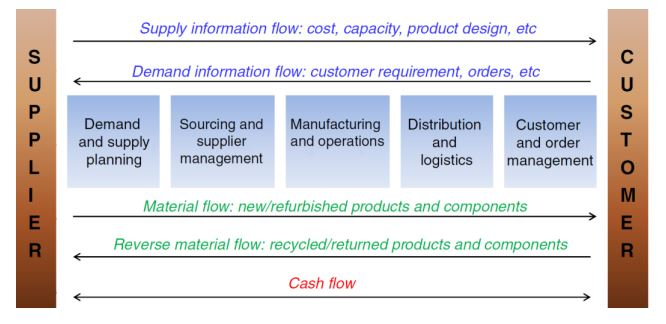
\includegraphics[width=.9\textwidth]{images/Alaa/supplyChain.JPG}%
     % you need to add the caption for the list of figures
    \caption[Supply chain process]{Supply chain process.}\label{fig: Supply chain process}%
  \end{figure}
  
While E-commerce includes online transactions business-to-business (B2B), business-to-consumer (B2C), consumer-to-business (C2B), and consumer-to-consumer (C2C), both with respect to virtual and physical goods, so it's dealing with the concept of delivery, to deliver the order to the requester. 

\section {Automating Delivery Process}
\hspace{2cm} Nowadays you can select and send your order to the market via software application and the delivery process will performed automatically, no need to go out from your room.
Autonomous vehicles are the next big thing in providing transportation solutions that are safer, cleaner and faster, so we can define autonomous vehicles as cars or trucks in which human drivers are never required to take control to safely operate the vehicle. Also known as “driverless” cars, they combine sensors and software to control, navigate, and drive the vehicle.\cite{web016}
\par
Automating delivery process helps to solve some problems and provides many benefits such as:
\begin{itemize}
    \item Providing safety and reducing car accidents and casualties immensely are benefits of automating the delivery process for the person who is delivering the orders.
    \item Making the delivery process as fast as possible to satisfy the client and save the customer's energy are benefits of automating the delivery process for the customer.
    \item provide paid salaries for drivers to be used on other things is one of benefits of automating the delivery process for the company.
    
\end{itemize}
While conventional delivery can increase the number of accidents as it is reported that 90 percent of car accidents are due to human error. In addition, conventional delivery process can take longer time until the order reaches to the requester, because the driver may be busy by making phone calls that will not only affect the delivery time but also will affect his safety.

\section{Use of Self-driving Cars in Delivery Systems}
\hspace{2cm} Self-driving car technology is advancing every day, and it's only a matter of time before fully driverless vehicles appear on public streets.
Almost daily, there's a new development in the driverless car space, and nearly every major car manufacturer, ride-sharing service and tech company from Apple to Google has bought into the driverless car industry. 
Self -driving car can be used in various and varied applications. The most common one is transferring someone from one place to another. It also can be used on indoor and outdoor delivery system to deliver items to the one who requested them. Now, we will consider some of the applications of self-driving car:
\par
\begin{itemize}
 \item\textbf{Apple self-driving cars}: Apple is actively testing its self-driving car tech, evidenced by several car sightings in the last few years. Though the vehicles lack proprietary markings, the cars are bedecked in all the gear needed to run self-driving systems and are often seen driving around Apple office buildings and into Apple complex parking lots. 
\par
Apple's self-driving cars are coming out of the shadows and onto public roads, but that's not all that's circulating about Apple's automotive project.
In May 2018, it was revealed by the California DMV that Apple's autonomous car permit now covers 55 cars and 83 drivers, giving it the second biggest autonomous car fleet in California.\cite{web029}
\begin{figure}[H]%
    \center%
    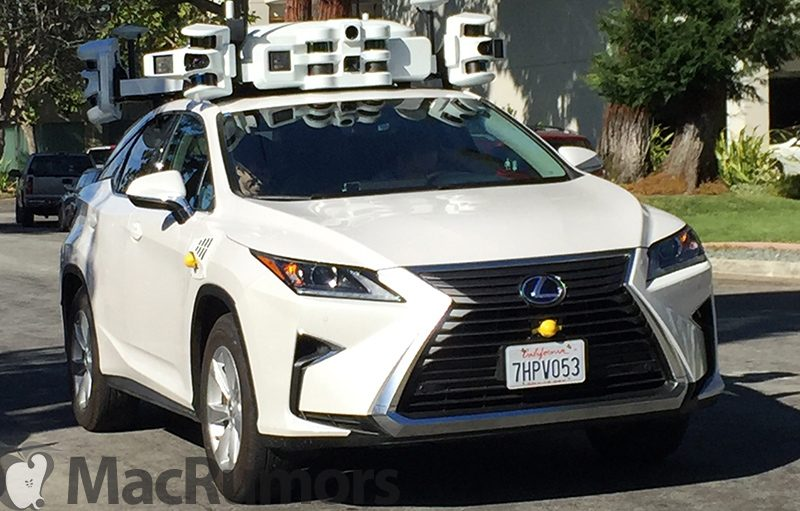
\includegraphics[width=.5\textwidth]{images/Alaa/apple.jpg}%
     % you need to add the caption for the list of figures
  \end{figure}
  
\item\textbf{Google's driverless cars }:
Waymo LLC is a self-driving technology development company. It is a subsidiary of Alphabet Inc. Waymo originated as a project of Google before it became a stand-alone subsidiary in December 2016. In April 2017, Waymo started a limited trial of a self-driving taxi service in Phoenix, Arizona. On December 5, 2018, the service launched a commercial self-driving car service called "Waymo One"; users in the Phoenix metropolitan area use an app to request a pick-up.\cite{web030}
\begin{figure}[H]%
    \center%
    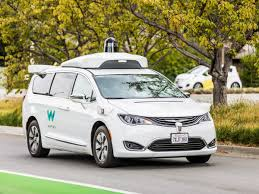
\includegraphics[width=.5\textwidth]{images/Alaa/waymo.jpg}%
     % you need to add the caption for the list of figures
  \end{figure}
  
\item\textbf{DoorDash delivery system }:
DoorDash announced it is partnering with General Motors' Cruise autonomous-vehicles unit to deliver food and groceries. The program will kick off early this year in the San Francisco area.
For now, a DoorDash delivery person will be present in the self-driving car and bring the groceries or meal to the doorstep. In the future, customers will be able to decide between picking up a delivery from the curb or via a fully autonomous delivery system.
The partnership is starting with one merchant and one vehicle, with plans to add more cars and merchants in the future.
Self-driving cars have been a growing presence in the food and grocery delivery business. Ford and Postmates announced plans to collaborate on a self-driving delivery service last June. Kroger partnered with robotics-company Nuro to deliver groceries in Scottsdale, Arizona. Domino's began testing self-driving cars in 2017.\cite{web031}

\par
\item\textbf{Olli car}: Olli is the world’s first self-driving, cognitive shuttle that uses IBM’s Watson technology to provide a more personalized experience. Olli is currently a “first mile/last mile” solution with the goal of being implemented in cities, towns and municipalities all over the world to solve congestion, pollution and accessibility issues. Olli currently would fill the service that a personal vehicle provides, allowing people to take Olli around town or from a transit station to their final destination.\cite{web032}

\begin{figure}[H]%
    \center%
    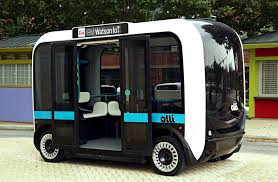
\includegraphics[width=.5\textwidth]{images/Alaa/olli.jpg}%
     % you need to add the caption for the list of figures
  \end{figure}
\end{itemize}


\section{History of Autonomous Delivery}
\hspace{2cm} Self-driving cars history dates back to the 1500s and has continued to this day. The chronological date of the self-driving cars will be shown since its inception:
\par
\begin{itemize}
\item \textbf{Da Vinci’s Self-Propelled Cart—c. 1500} Centuries before the invention of the automobile, Leonardo da Vinci designed a cart that could move without being pushed or pulled. Springs under high tension provided the power to the cart, and steering could be set in advance so the cart could move along a predetermined path. A distant precursor to the car, the device is sometimes considered the world’s first robot.

\par
\item \textbf{Whitehead Torpedo—1868} While these weapons of war emerged in the mid-1700s, Robert Whitehead’s invention of a torpedo that could propel itself underwater proved to be a game-changer for naval fleets around the world. The Whitehead torpedo could travel several hundred yards underwater and maintain depth, thanks to a pressurization system dubbed “The Secret.” Torpedo guidance would evolve dramatically thereafter and led to a wide range of weaponry, aircraft, and other autonomous devices.

\par
\item \textbf{Mechanical Mike Aircraft Autopilot—1933 } Extended travel times forced the development of autopilot systems for long-range aircraft. Mechanical Mike was a prototype autopilot designed by Sperry Gyroscope Co., and used by Wiley Post during a 13,000-mile, around-the-world flight in 1933. Gyroscopes kept track of the plane’s heading and interfaced with the controls to ensure accurate direction. Gyroscopes remain an integral part of autonomous vehicle tech today.

\par
\item \textbf{Teetor Cruise Control—1945} An engineer became so fed up with the rocking motion he experienced while riding in a car with his attorney behind the wheel that he developed one of the first cruise control system to smooth out the ride, using a mechanical throttle that could set the vehicle’s speed. The invention was commercialized in 1958.

\par
\item \textbf{Tsukuba Mechanical Engineering—1977 } As groundbreaking as the Stanford Cart was, it was still just a four-wheeled cart that looks more at home in the kitchen than on a roadway. Japan-based Tsukuba Mechanical produced an autonomous passenger vehicle that could recognize street markings while traveling at nearly 20 miles per hour, thanks to two vehicle-mounted cameras.

\par
\item \textbf{VaMoRs—1987} Another important step forward in autonomous tech came from German engineer Ernst Dickmanns, who equipped a sedan with a bank of cameras and 60 micro-processing modules to detect objects on the road—in front of and behind the vehicle.

\par
\item \textbf{General Atomics MQ-1 Predator—1995}  While we tend to think of autonomous vehicles as a means of converting humans from drivers to passengers, another class of autonomous devices are designed to travel completely alone. Nowhere is this more visible than in the world of drones, the most noteworthy of which has been General Atomics’ Predator, an unmanned plane that for 20 years has been piloting over global hotspots for 14 hours at a time. Drones aren’t just military vehicles, of course. The Predator is decked out with technologies being adapted for cars, including radar that can see through smoke or clouds and thermal imaging cameras that enable travel by night.

\par
\item \textbf{DARPA Challenges—2004-2013}  The U.S. Department of Defense’s research arm, DARPA, sponsored a series of challenges that pushed autonomous technologies forward. In 2004, a competition was held to challenge vehicles to self-navigate 150 miles of desert roadway. While no car completed the route, subsequent challenges have seen dramatic leaps in capabilities. The 2007 challenge simulated a 60-mile long urban environment, with four cars completing the route in the allotted six-hour time limit.

\par
\item \textbf{Tesla Autopilot—2015} The most significant aspect of Tesla’s semi-autonomous “Autopilot” feature, introduced in late 2015—which enabled hands-free control for highway and freeway driving— is that it was delivered in the form of a single software update to Model S owners overnight.\cite{web028}
\end{itemize}

\section{Related Products}
\hspace{2cm} Many companies generated self driving car and employed it in different applications, we will discuss some of them according to 2018 :
\par

\begin{itemize}
 \item \textbf{Nuro}: 
Nuro was founded by two former lead Google engineers, Dave Ferguson and Jiajun Zhu, who previously worked on the Google’s self-driving car project. They are designing a self-driving, small delivery vehicle which will travel on roads and focus on low-speed, local, and last-mile deliveries: groceries, laundry, packages or your take-out order. Rather than adapting existing vehicles designs to fit their model, their engineers have instead built something entirely new from scratch. Nuro’s first prototype has a “handle” on the roof which serves as a platform for the vehicle’s array of sensors — including LIDAR, cameras, and radars. Its self-driving status eliminates the need for all the normal inner components of a car — such as the steering wheel and driving seat — and means that the vehicle’s inner space can be dedicated solely to delivery lockers. Nuro is using a fleet of six self-driving cars to collect data and optimize routes, which will then be fed into its prototype vehicles. It has received a permit from the California DMV and plans to start testing on public roads later this year.\cite{web027}

\begin{figure}[H]%
    \center%
    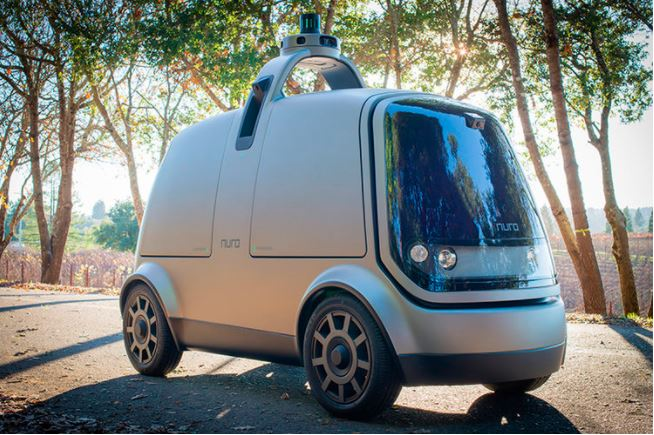
\includegraphics[width=.5\textwidth]{images/Alaa/nuro.JPG}%
  \end{figure}

\par
 \item \textbf{Robomart } : 
Robomart advertises itself as the ‘world’s first self-driving store’. Unlike other delivery services which focus on delivering goods pre-bought online, Robomart is quite literally a moving fresh produce store, bringing vegetables to people’s doors and allowing them to pick what they want on the spot. Similar to Uber and other taxi apps, customers tap a button to request the closest robomart circulating in their local area. Once it arrives, they head outside, unlock the doors, and shop for the products they want, closing the doors when they’re done and sending it on its way. \cite{web027} 

\begin{figure}[H]%
    \center%
    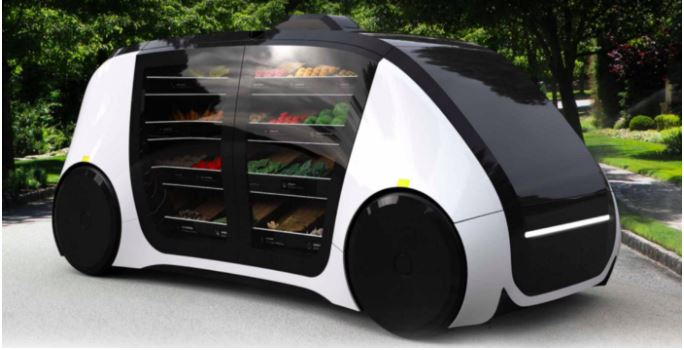
\includegraphics[width=.5\textwidth]{images/Alaa/robomart.JPG}%
  \end{figure}

\par
 \item \textbf{Delivery with Normal Autonomous cars} :
Nearly all major food delivery companies are playing with the idea of delivery through normal, autonomous vehicles. For example, Ford invested 1 billion dollar investment in artificial intelligence company Argo A.I. in 2017 and is now testing an autonomous pizza delivery vehicle in Miami in partnership with Domino’s. Toyota and Pizza Hut have also joined forces to ‘make pizza delivery more efficient’. \cite{web027}

\par
 \item \textbf{Gita }:
Gita is a round, mobile-carrier that follows people on the go; it was designed by PFF, a subsidiary of Piaggio Group that was created in 2015 to research and develop lightweight, intelligent mobility solutions for people and goods. Gita learns to navigate complex spaces by trailing its human owner and can carry up to 44 pounds of cargo and a volume of up to nearly 2,000 cubic inches (the equivalent of a case of wine, a loaded backpack, or two stuffed grocery bags). Gita is not therefore an autonomous delivery robot as such, but rather a kind of self-driving ‘moving bag’, that helps those with a mobile lifestyle — from millennials and parents to seniors and disabled individuals — to carry more than they could on their own.\cite{web027}
\begin{figure}[H]%
    \center%
    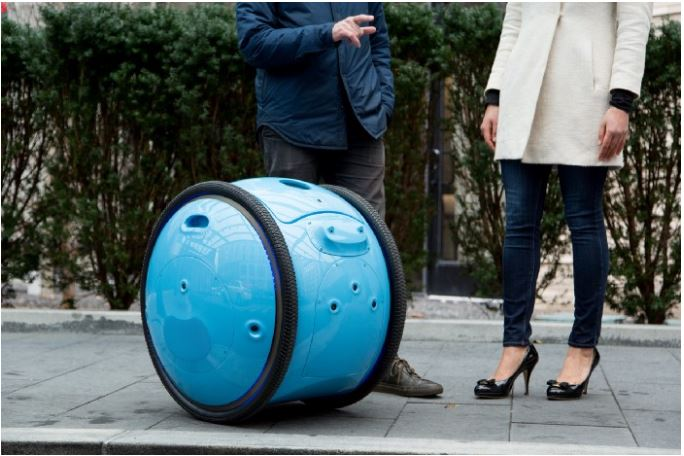
\includegraphics[width=.5\textwidth]{images/Alaa/gita.JPG}%
  \end{figure}


\par
 \item \textbf{Amazon Prime Air}:
Amazon Prime Air is a delivery system developed by Amazon that is designed to safely deliver packages to customers using unmanned aerial vehicles (a.k.a, drones). Customers choose from a selection of items in an Amazon fulfilment centre near their homes and just moments after they order, an Amazon drone makes it way down an automated track and lifts off into the open sky, heading to its destination completely on its own. Travelling at a height of roughly 400ft, carrying packages up 5 pounds, guided by GPS and using so-called ‘sense-and-avoid’ technologies, these drones deliver packages in under 30 minutes. \cite{web027}
\begin{figure}[H]%
    \center%
    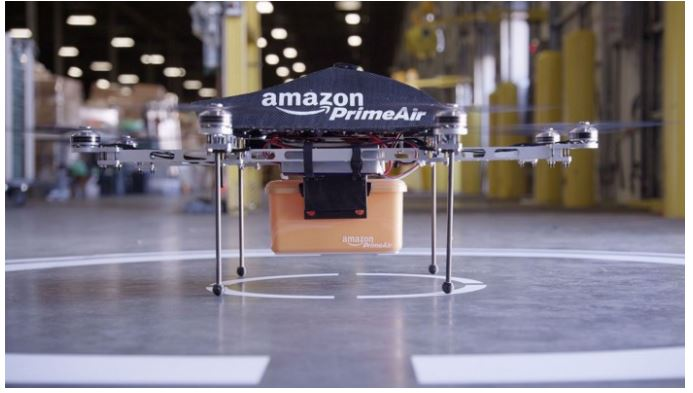
\includegraphics[width=.5\textwidth]{images/Alaa/prime.JPG}%
  \end{figure}
\end{itemize}

\section{Project Scope}
\hspace{2cm} Last mile delivery is an important term in the communities of supply chain management and e-commerce. It refers to transferring goods and materials from a transportation hub to their final destinations at homes. In this project we propose a fully autonomous robotic system for last mile delivery applications. The proposed system is supposed to perform two main functions. The first function is connecting clients purchasing different objects with the vendors supplying these objects in a certain area. The second function is transferring purchased objects to their final destinations. We aim to develop a self-driving robot that is capable of safely transferring objects in noisy and crowded outdoor environments.

Our work to complete this project is divided into three milestones:
 \begin{itemize}
\item   Build a self-driving robot which is supposed to perform the following tasks:
    \begin{itemize}
    \item Low level motion control.
    \item Obstacle avoidance during motion.
    \item Path tracking to reach destination.
    \item Localization
    \item Sensor Fusion using sensors besides robot odometry to increase accuracy of localization process.
    \end{itemize}
\item  Develop a web server to perform the following tasks:
    \begin{itemize}
    \item Monitor all the robots in the system.
    \item Keep track of vendors using our service and their products.
    \item Path planning to determine the way for robots.
    \end{itemize}
\item  Design a suitable user interface for vendors, who use our service to transfer their products to purchasers, and clients shipping their groceries through our service.

\end{itemize}

%%%%%%%%%%%%%%%%%%%%%%%%%%%%%%%%%%%%%%%%%%%%%%%%%%%%%%%%%%%%%%%%%%%%%%%%%%%%%%%%%%%%%%%%%%%%%%%%%%%%%%%%%%%%%%%%%%
%%%%%%%%%%%%%%%%%%%%%%%%%%%%%%%%%%%%%%%%%%%%%%%%%%%%%%%%%%%%%%%%%%%%%%%%%%%%%%%%%%%%%%%%%%%%%%%%%%%%%%%%%%%%%%%%%%
    \cleardoublepage%
        
     %%%%%%%%%%%%%%%%%%%%%%%%%%%%
% CHAPTER                  %
%%%%%%%%%%%%%%%%%%%%%%%%%%%%
\chapter{System Components and Architecture}%
\label{chap:chap2}

%%%%%%%%%%%%%%%%%%%%%%%%%%%%
% SECTION                  %
%%%%%%%%%%%%%%%%%%%%%%%%%%%%
\newline
\newline
\vspace{3mm}
\hfill
\section{Introduction}
\hspace{2cm} In this chapter we present an overview of the whole system components, their architecture, usage and how they are connected. We also present system modules that perform the functionality of the system and how they are integrated together. And a business scenario that recaps the flow of the project.

\section{Hardware Components}
\subsection{Robot Platform}
\hspace{2cm}The platform we use in our project is 6-wheel-drive chassis from Dagu Electronics has independent suspension for each of its spiked 120mm-diameter wheels, allowing exceptional traction over uneven terrain, and its body is made from 2mm-thick anodized aluminum with a 10mm-pitch grid of 4mm holes, making it easy to mount electronics and accessories to the chassis. Assembly of the chassis is a simple three-step process that takes just minutes. This model has 75:1 steel gearboxes on the motors, see figure \ref{fig:wild thumper}. The robot the following architecture: \cite{web012}
 \begin{itemize}
        \item Size: 420 x 300 x 130 mm
        \item Weight: 2.7 kg
        \item Recommended motor voltage: 2 - 7.5 V
        \item Metal gearmotor: 25D mm
        \item Dagu wheel (chrome) with Pololu: 120 x 60 mm
    \end{itemize}{}

 \begin{figure}[H]%
    \center%
    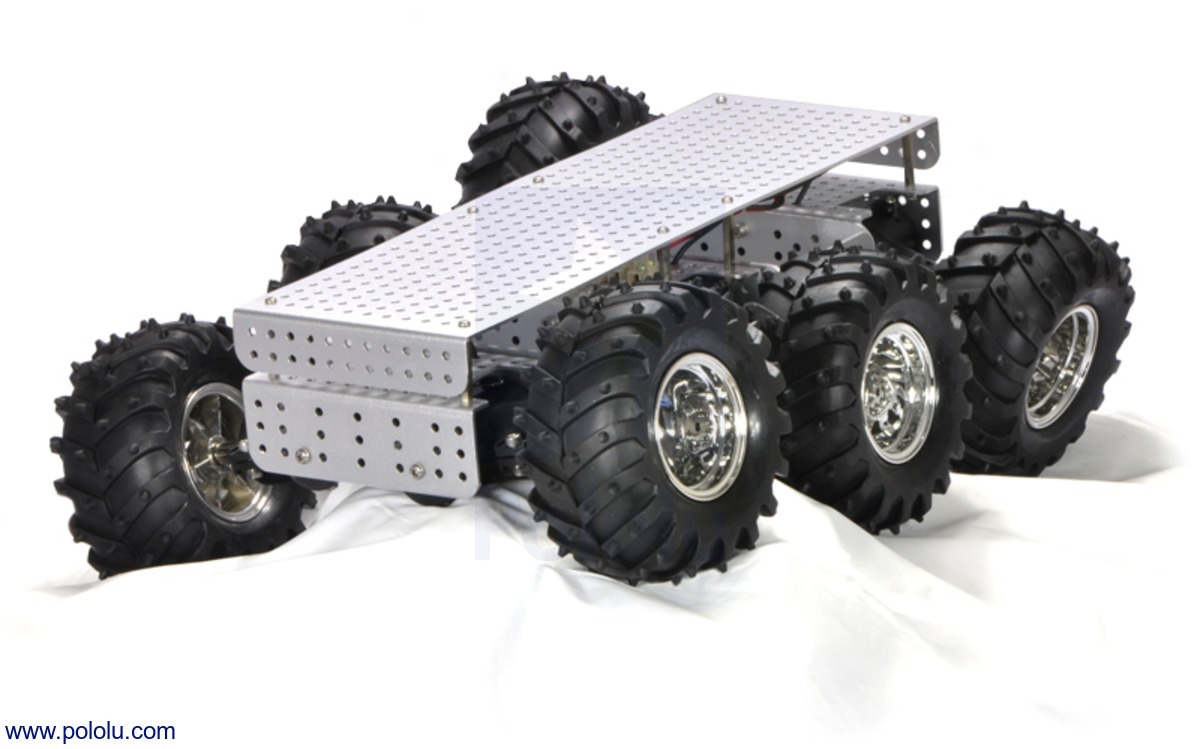
\includegraphics[width=.8\textwidth]
    {images/Alzahraa/wild_thumper.jpg}%
    \caption[Wild Thumper]{Wild Thumper 6 WD}\label{fig:wild thumper}%
  \end{figure} 

\subsection{Motor Drivers}
\hspace{2cm}Motor drives are circuits used to run a motor. In other words, they are commonly used for motor interfacing. These drive circuits can be easily interfaced with the motor and their selection depends upon the type of motor being used and their ratings (current, voltage).\cite{web013}\\
In our project we use two BTS7960 KIT (see figure \ref{fig:motor drivers}) having the following architecture:
\begin{itemize}
    \item High-power drive full H-bridge driver module with thermal over-current protection.  High-current 43A.
    \item Double BTS7960 large current (43 A) H bridge driver.
    \item 5V isolate with MCU, and effectively protect MCU.
    \item 5V power indicator on board.
    \item Voltage indication of motor driver output end.
    \item Heat sink can be added. 
    \item Isolation chip 5 V power supply (can share with MCU 5 V).
    \item Size: 4 * 5 * 1.2 cm.
    \item Ability to reverse the motor forward, two PWM input frequency up to 25kHZ.
    \item Two heat flow passing through an error signal output.
    \item Isolated chip 5V power supply (can be shared with the MCU 5V), can also use the on-board 5V supply.
    \item The supply voltage 5.5V to 27V. 
\end{itemize}
Both drivers are powered by LIPO 7.4V -4200mAh battery.

\begin{figure}[H]%
    \center%
    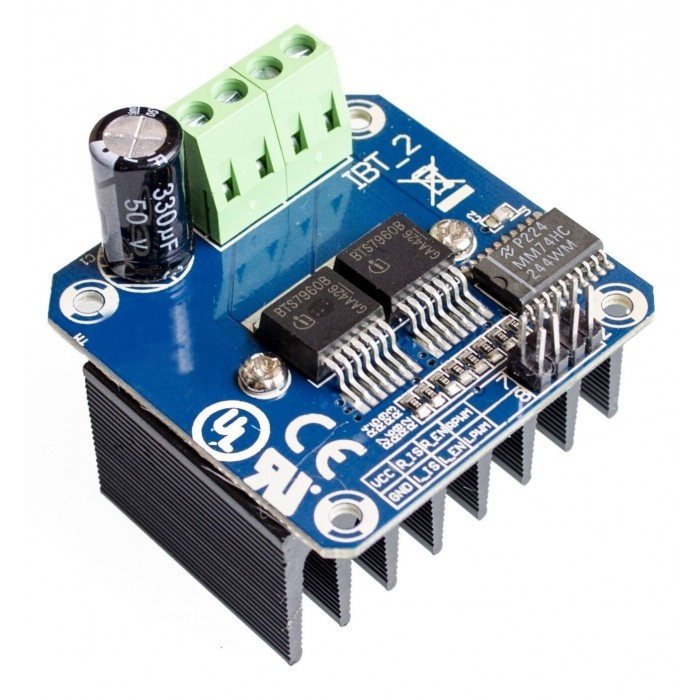
\includegraphics[width=.5\textwidth]
    {images/Alzahraa/motor_drivers.jpg}%
    \caption[Motor Driver]{Motor driver BTS7960}\label{fig:motor drivers}%
  \end{figure} 

\subsection{Arduino}
\hspace{2cm}Arduino is an open-source hardware and software company, project and user community that designs and manufactures single-board microcontrollers and microcontroller kits for building digital devices and interactive objects that can sense and control both physically and digitally.
Arduino board designs use a variety of microprocessors and controllers. The boards are equipped with sets of digital and analog input/output (I/O) pins that may be interfaced to various expansion boards or breadboards (shields) and other circuits. The boards feature serial communications interfaces, including Universal Serial Bus (USB) on some models, which are also used for loading programs from personal computers. The microcontrollers are typically programmed using a dialect of features from the programming languages C and C++. In addition to using traditional compiler toolchains, the Arduino project provides an integrated development environment (IDE) based on the Processing language project.\cite{web017} 
In our project we use Arduino UNO (see figure \ref{fig:arduino uno}) having the following architecture: \\
\begin{itemize}
    \item Microcontroller board based on the ATmega328P.
    \item 14 digital input/output pins (of which 6 can be used as PWM outputs), 6 analog inputs, a 16 MHz quartz crystal, a USB connection, a power jack, an ICSP header and a reset button.\cite{web014}\\
\end{itemize}
\begin{figure}[H]%
    \center%
    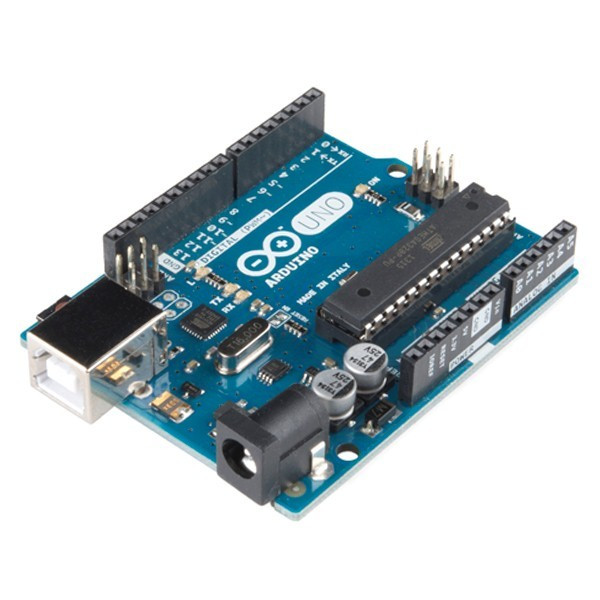
\includegraphics[width=.5\textwidth]
    {images/Alzahraa/arduino_uno.jpg}%
    \caption[Arduino Uno]{Arduino UNO}\label{fig:arduino uno}%
  \end{figure} 

\subsection{Raspberry Pi}
\hspace{2cm}A Raspberry Pi is a credit card-sized computer originally designed for education, inspired by the 1981 BBC Micro. Creator Eben Upton’s goal was to create a low-cost device that would improve programming skills and hardware understanding at the pre-university level. But thanks to its small size and accessible price, it was quickly adopted by tinkerers, makers, and electronics enthusiasts for projects that require more than a basic microcontroller.
The Raspberry Pi is slower than a modern laptop or desktop but is still a complete Linux computer and can provide all the expected abilities that implies, at a low-power consumption level. \cite{web006} \\
In our project we use Raspberyy Pi 3 model B (see figure \ref{fig:raspberryPi}) having the following architecture:
\begin{itemize}
    \item Quad Core 1.2GHz Broadcom BCM2837 64bit CPU.
    \item 1GB RAM.
    \item BCM43438 wireless LAN and Bluetooth Low Energy (BLE) on board.
    \item 100 Base Ethernet.
    \item 40-pin extended GPIO.
    \item 4 USB 2 ports.
    \item 4 Pole stereo output and composite video port.
    \item Full size HDMI.
    \item CSI camera port for connecting a Raspberry Pi camera.
    \item DSI display port for connecting a Raspberry Pi touchscreen display.
    \item Micro SD port for loading your operating system and storing data.
    \item Upgraded switched Micro USB power source up to 2.5A.\cite{web018}
\end{itemize}

\begin{figure}[H]%
    \center%
    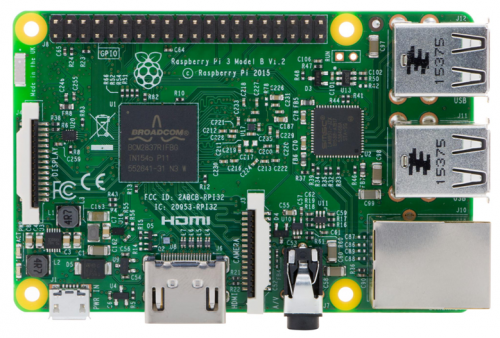
\includegraphics[width=.5\textwidth]
    {images/Alzahraa/raspberryPi.png}%
    \caption[Raspberry Pi]{Raspberry Pi 3 model B}\label{fig:raspberryPi}%
  \end{figure} 


\subsection{Sensors}
\hspace{2cm}A sensor is a device, module, or subsystem whose purpose is to detect events or changes in its environment and send the information to other electronics, frequently a computer processor. \cite{web007} \\
Sensors used in our project are:
\begin{enumerate}
   \item IMU: \\
   An inertial measurement unit (IMU) is an electronic device that measures and reports a body's specific force, angular rate, and sometimes the orientation of the body, using a combination of accelerometers, gyroscopes, and sometimes magnetometers. \cite{web008}\\
   In Our project we use Adafruit 9-DOF IMU module (see figure \ref{fig:fig:adafruit}) having the following architecture:

    \begin{itemize}
        \item Dimensions: 20mm x 27mm x 4mm / 0.8" x 1.1" x 0.2"
        \item Header holes begin 4mm from the mounting holes
        \item Mounting Hole dimensions: 20mm x 12mm apart
        \item Uses I2C address 0x28 (default) or 0x29
        \item Weight: 3g 
    \end{itemize}{}

   \begin{figure}[H]%
    \center%
    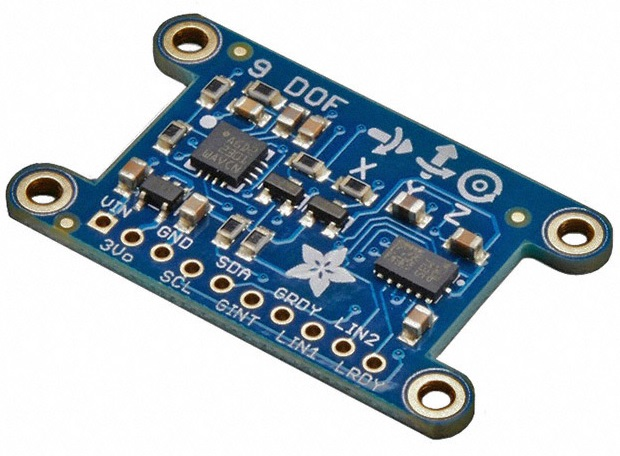
\includegraphics[width=.5\textwidth]
    {images/Alzahraa/imu_Adafruit.jpg}%
    \caption[IMU Adafruit]{Adafruit 9-DOF IMU}\label{fig:adafruit}%
  \end{figure}
   
   \item GPS: \\
   The Global Positioning System (GPS), is a satellite-based radionavigation system owned by the United States government and operated by the United States Air Force. It is a global navigation satellite system that provides geolocation and time information to a GPS receiver anywhere on or near the Earth where there is an unobstructed line of sight to four or more GPS satellites. Obstacles such as mountains and buildings block the relatively weak GPS signals. \cite{web009}\\
   In Our project we use DIYmall NEO-6M GPS module (see figure \ref{fig:neo_6m}) having the following architecture:
    \begin{itemize}
        \item Standalone GPS receiver
        \item U-blox NEO-6M GPS module 
        \item Under 1 second time-to-first-fix for hot and aided starts
        \item SuperSense ® Indoor GPS: -162 dBm tracking sensitivity
        \item Anti-jamming technology
        \item Support SBAS (WAAS, EGNOS, MSAS, GAGAN)
        \item u-blox 6 50 channel positioning engine with over 2 million effective correlators
        \item Timepulse
        \item 5Hz position update rate
        \item Operating temperature range: -40 TO 85°C
        \item UART TTL socket 
        \item EEprom to store settings
        \item Rechargeable battery for Backup 
        \item Build in 18X18mm GPS antenna 
        \item RoHS compliant 
    \end{itemize}{}
     \begin{figure}[H]%
    \center%
    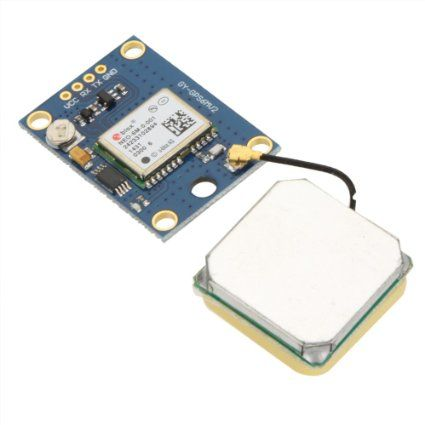
\includegraphics[width=.5\textwidth]
    {images/Alzahraa/gps_NEO_6M.jpg}%
    \caption[GPS NEO]{DIYmall NEO-6M GPS}\label{fig:neo_6m}%
  \end{figure}
   
   \item LIDAR: \\
   Lidar is a surveying method that measures distance to a target by illuminating the target with pulsed laser light and measuring the reflected pulses with a sensor. Differences in laser return times and wavelengths can then be used to make digital 3-D representations of the target. The name lidar, now used as an acronym of light detection and ranging (sometimes light imaging, detection, and ranging), was originally a portmanteau of light and radar. Lidar sometimes is called 3D laser scanning, a special combination of a 3D scanning and laser scanning. It has terrestrial, airborne, and mobile applications. \cite{web010}\\
   In Our project we use YDLIDAR Lidar F4  2D Lidar scanner (see figure \ref{fig:ydlidar}) having the following architecture:
    
    \begin{itemize}
        \item Application field:Environment Scanning, SLAM Application and Robot Navigation
        \item 360-degree laser rangefinder, Scanner range 12 Meter,MAX. 6000Hz Ranging Sample rate
        \item OS: Windows, Android, ROS and Linux,Ultra long working life,Weight: 189g
        \item F4 uses Industrial Brushless Moto,Scanning Rate: 6000tims/s,Laser grade: Class 1,Configurable Scanning Frequency: 5-12Hz
        \item Quick Start-F4 has complete drivers as well as complete SDK ,API and documentation. It's easy for users to get started quickly.
    \end{itemize}{}
    
     \begin{figure}[H]%
    \center%
    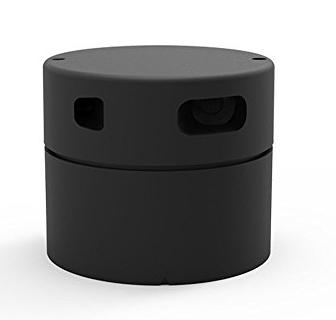
\includegraphics[width=.5\textwidth]
    {images/Alzahraa/lidar_ydlidar.jpg}%
    \caption[YDLIDAR LIDAR]{YDLIDAR Lidar F4  2D Lidar scanner}\label{fig:ydlidar}%
  \end{figure}
   
    \item Webcam: \\
  A webcam is a small digital video camera directly or indirectly connected to a computer or a computer network. \cite{web011}\\
   In Our project we use 1080P Nano Shield N920 Webcamera (see figure \ref{fig:nano_webcam}) having the following architecture:
   
   \begin{itemize}
        \item Premium auto focus and light correction.
        \item Full HD 1080P at 30 fps recording.
        \item Noise cancelling microphone.
        \item Tripod ready mount.
        \item IM compatibility. 
   \end{itemize}{}
   
   \begin{figure}[H]%
    \center%
    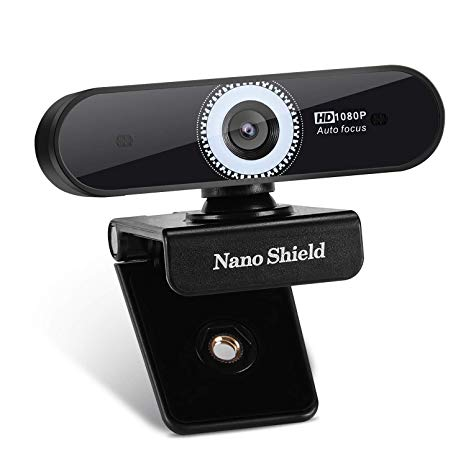
\includegraphics[width=.5\textwidth]
    {images/Alzahraa/webcamera_nano.jpg}%
    \caption[Camera Nano]{1080P Nano Shield N920 Webcamera}\label{fig:nano_webcam}%
  \end{figure}
   \end{enumerate}
   
%%%%%%%%%%%%%%%%%%%%%%%%%%%%%%%%%%%%%%%%%%%%%%%%%%%%%%%%%%%%%%%%%%%%%%%%%%%%
   \section{Software Components}
\subsection{Web Sever}
\hspace{2cm}The aim of this part is to develop website that process requests and delivers data from and to clients over the internet or a local network. A web-based interface is developed for clients to interact with the system. 

\subsection{Robot Software Platform}
\hspace{2cm}We integrate all components of the robot platform using Robot Operating System (ROS). The aim of this part is to provide low-level device control, connect all processes together and provide message-passing between processes with no effort. 
\section{System Architecture}
\hspace{2cm}To achieve its goal, our project is divided into several main modules which are integrated together in an appropriate manner, these modules are as follows:\\
\begin{enumerate}
    \item Web server
    \item Path planning
    \item Neural network 
    \item Main controller
    \item Convolutional Neural Network
    \item Classical control
    \item Obstacle avoidance
    \item Localization 
\end{enumerate}
These modules work on data from IMU, GPS, LIDAR and Webcam then send actions to Arduino to perform the tasks required by the client. An overview of the architecture is shown below in figure \ref{fig:system_arch}

  \begin{figure}[H]%
    \center%
    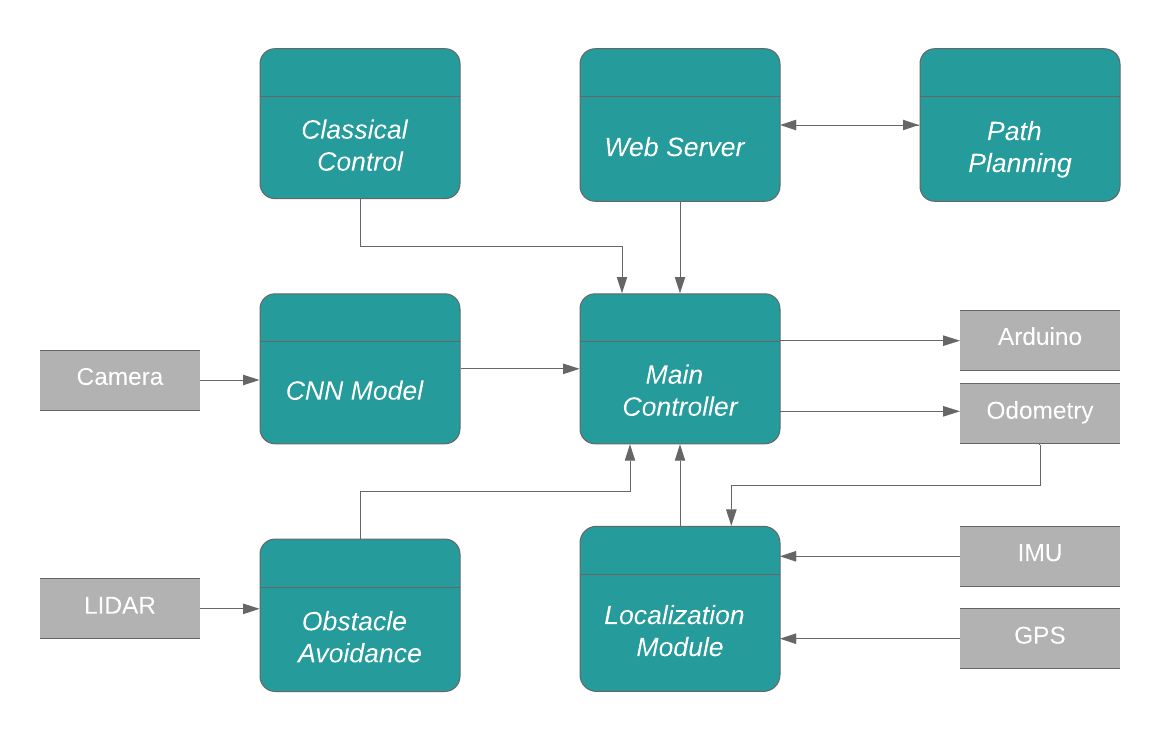
\includegraphics[width=\textwidth]
    {images/Alzahraa/system_arch.png}%
     % you need to add the caption for the list of figures
    \caption[System Architecture]{System Architecture}\label{fig:system_arch}%
  \end{figure}
  
\subsection{Web Server}
\hspace{2cm}The Web Service process resides on the web server. After the customer’s order is processed by the backend on the web server, An HTTP POST request is made to web server on the main device containing the task data.

\subsection{Path Planning}
\hspace{2cm}The path planning module takes the source and destination locations and generates the best path between them as several continuous nodes, then it sends the path to the main controller through the web server.

\subsection{Main Controller}
 \hspace{2cm}The main controller takes in all the control actions from CNN, classical control, obstacle avoidance modules and based on the current information provided from localization and path planning modules, it determines which control action will be sent to Arduino. 

\subsubsection{Convolutional Neural Network}
\hspace{2cm}The CNN (Neural Network) Module takes camera data as input and feeds raw images into the CNN. The details of the CNN module that used in our system is fully is discussed in chapter \ref{chap:chap5}. After processing the image the module outputs the predicted control action corresponding to that image and sends it to the main controller using an open socket connection. CNN model is used only to follow lane where there is no intersections.

\subsubsection{Classical Control}
\hspace{2cm}The classical control is used to generate actions at intersection points based on current and next poses of the robot that is being known from path planning and sends it to the main controller.

\subsubsection{Obstacle Avoidance}
\hspace{2cm}The Obstacle Avoidance module takes LIDAR data as input containing ranges and distances, then if the distance is below a certain threshold it outputs a high-priority control action, that is sent to the main controller.

\subsection{Localization}
\hspace{2cm}The localization module takes input: IMU, GPS and Odometry data, after processing the data using “Sensor Fusion” and “Extended Kalman Filter”  method, which is fully discussed in chapter \ref{chap:chap5}. It outputs an estimated location of the robot, that is sent to the main controller over a socket connection.

 
 \section{Business Scenario}
 \hspace{2cm}The delivery process starts when a customer decides to buy any product online using one of our services as follow:
 \begin{itemize}

     \item The customer's process starts by visiting the website or using the mobile application, searching for his required product, completing the ordering and payment process and inserting his location.
     \item The web server module receives the order created by customer and sends the locations of the customer and the vendor's that sells the required product to the path planning module.
     \item The path planning module generates three different paths and send them to the web server, the first is a path from the robot's base to the vendor's location, the second is from the vendor's location to the customer's location and the third is from the customer's location and back to the robot's base. 
     \item The web server sends the paths to the main controller, which parses them and gets ready for applying each individual path. 
     \item The CNN model generates an action depending on the image captured by the camera while moving and sends the action to the main controller.
     \item The classical control generates an action at intersections points and sends it to the main controller.
     \item The obstacle avoidance module generates an action and sends it to the main controller in case of existing obstacle.
     \item The main controller handles the three received actions and depending on the state of the robot it selects one of them and sends it to low-level control.
     \item The localization module generates an estimated location of the the robot current state and sends it to the main controller.
     \item The robot is said to be arrived at destination when the estimated location is the same as the final node in the current path. 
     \item The main controller notifies the web server for each arrival state.
     \item The vendor will be notified for the robot arrival in case of path 1, he packages the product and place it on the robot to be delivered.
     \item The customer will be notified for the robot arrival in case of path 2, it is time to get his order delivered.
     \item The robot uses the last path to return back to its robot base.
 \end{itemize}
 
 
  \begin{figure}[H]%
    \center%
    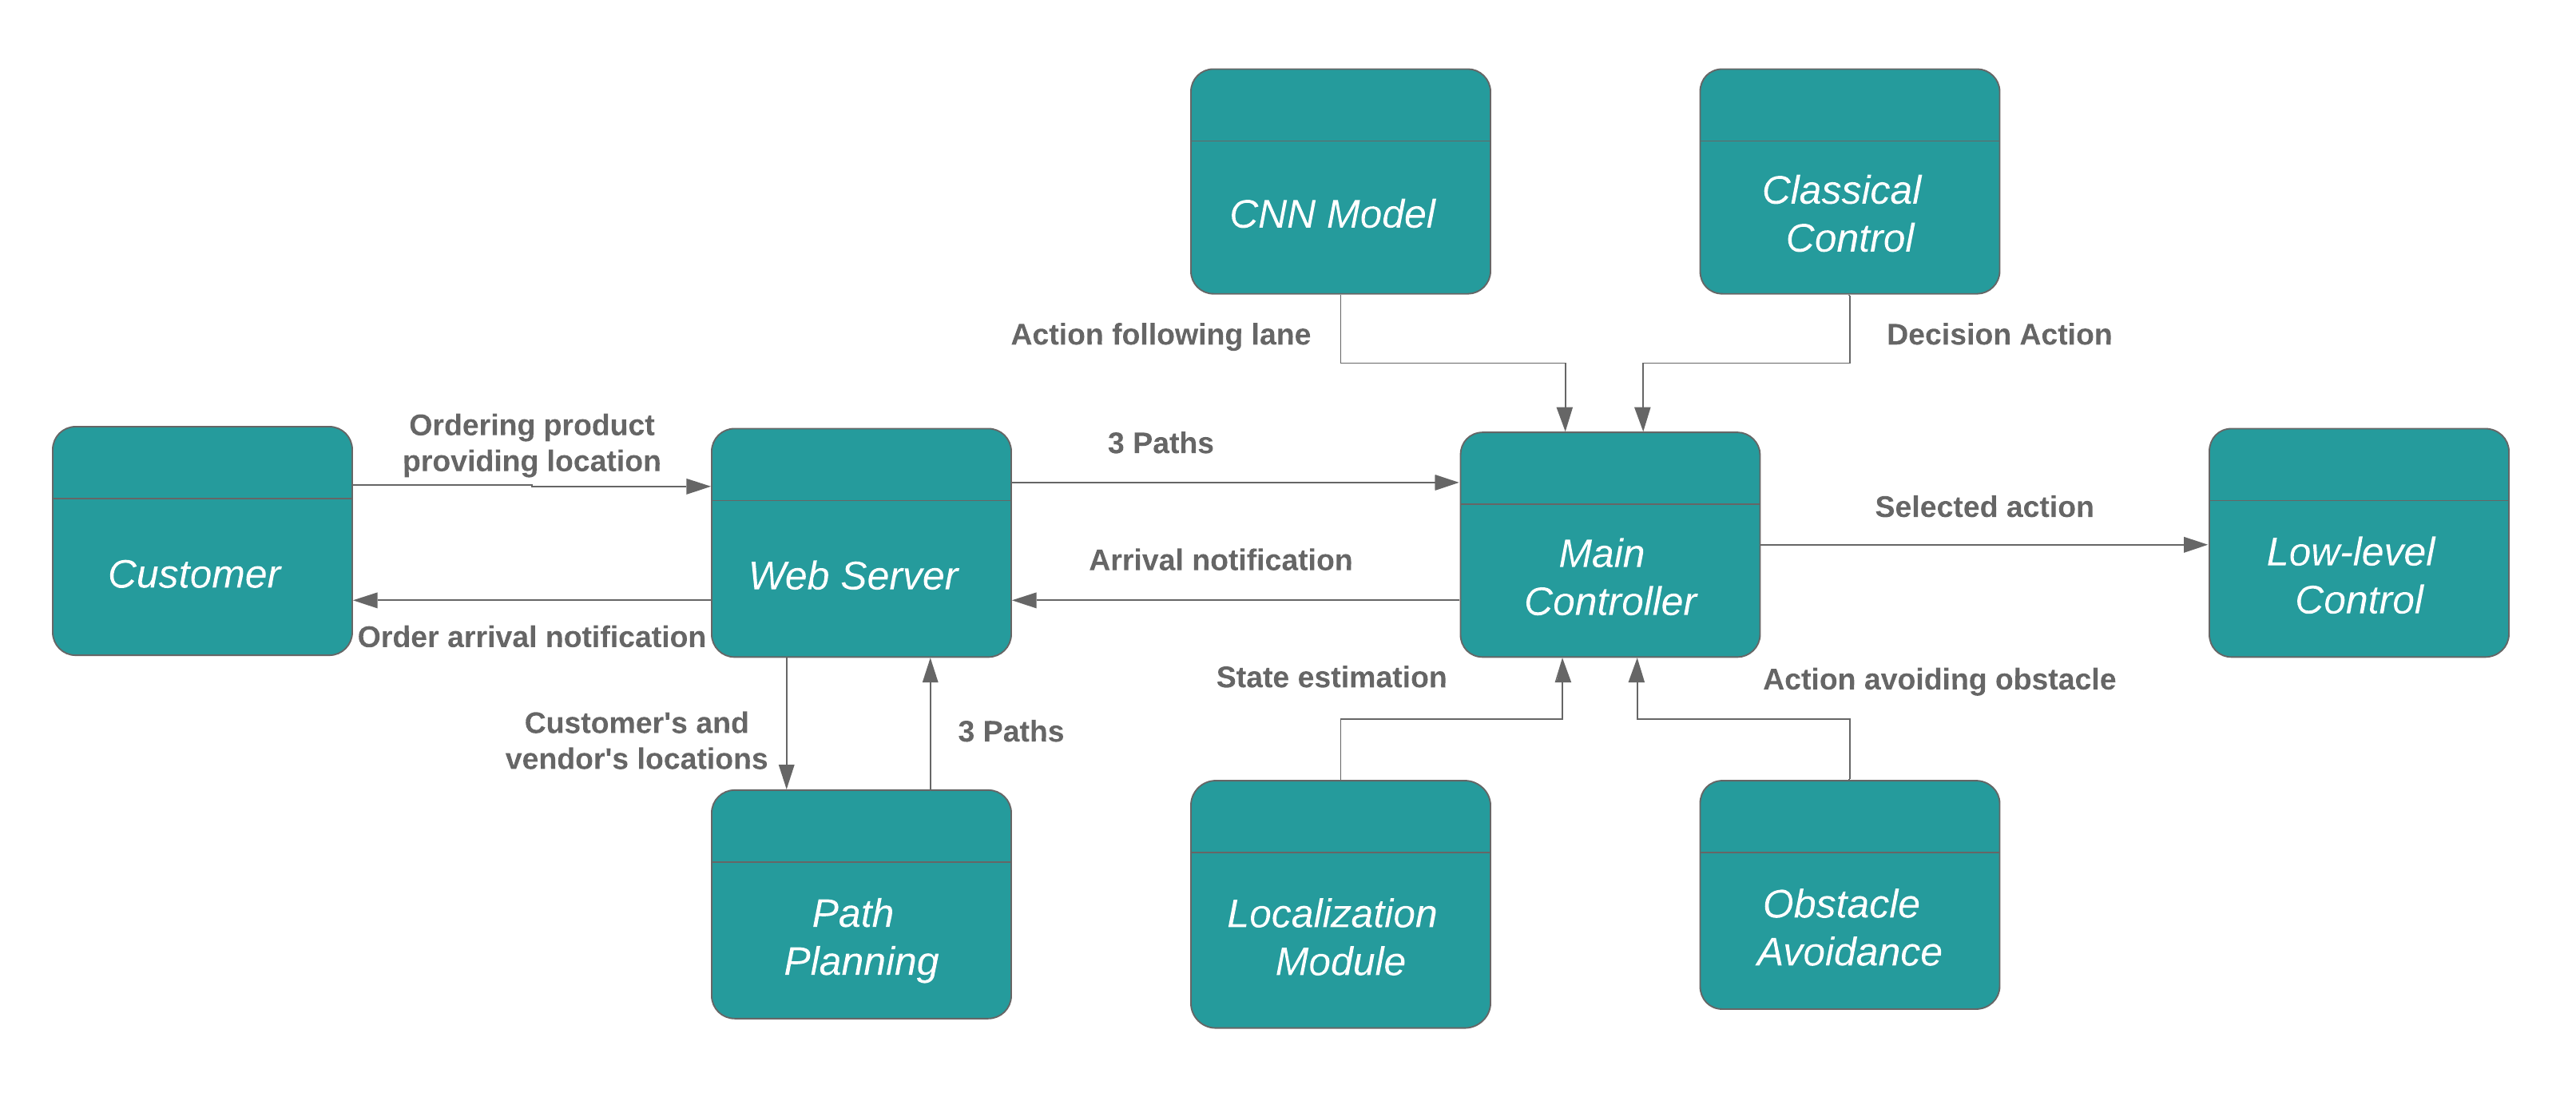
\includegraphics[width=\textwidth]
    {images/Alzahraa/business_scenario.png}%
     % you need to add the caption for the list of figures
    \caption[Business Scenario]{Business scenario}\label{fig:business scenario}%
  \end{figure}


%%%%%%%%%%%%%%%%%%%%%%%%%%%%%%%%%%%%%%%%%%%%%%%%%%%%%%%%%%%%%%%%%%%%%%%%%%%%%%%%%%%%%%%%%%%%%%%%%%%%%%%%%%%%%%%%%%
     \cleardoublepage%
    
     %%%%%%%%%%%%%%%%%%%%%%%%%%%%
% CHAPTER                  %
%%%%%%%%%%%%%%%%%%%%%%%%%%%%
\chapter{Robot Software Platform}%    %name of chapter that will appear
\label{chap:chap3}

%%%%%%%%%%%%%%%%%%%%%%%%%%%%
% SECTION                  %
%%%%%%%%%%%%%%%%%%%%%%%%%%%%
\newline
\newline
\vspace{3mm}
\hfill
\section{Introduction}
\hspace{2cm}In this chapter we will rather take a higher approach to our system, introducing our main software platform (ROS), which is considered as the beating heart of our system, then we illustrate the flow of data between the various system components. For the rest of this chapter we introduce our work environment on Raspberry Pi 3.

\section{Robot Operating System (ROS)}

\subsection{Introduction to ROS}
\hspace{2cm}ROS is an open source meta-operating system that runs on Unix operating systems, such as Linux Ubuntu. Similar to a regular operating system, it can provide low-level device control and message-passing between processes, but it is not designed to be the main operating system of a device. Since ROS is open source, it includes many online repositories from other organizations or community of developers, including industrial applications. ROS run-time graph is a peer-to-peer network of processes (potentially distributed across machines) that are loosely coupled using the ROS communication infrastructure. ROS implements several different styles of communication, including synchronous RPC-style communication over services, asynchronous streaming of data over topics, and storage of data on a Parameter Server.\cite{web040}

\begin{figure}[H]%
    \center%
    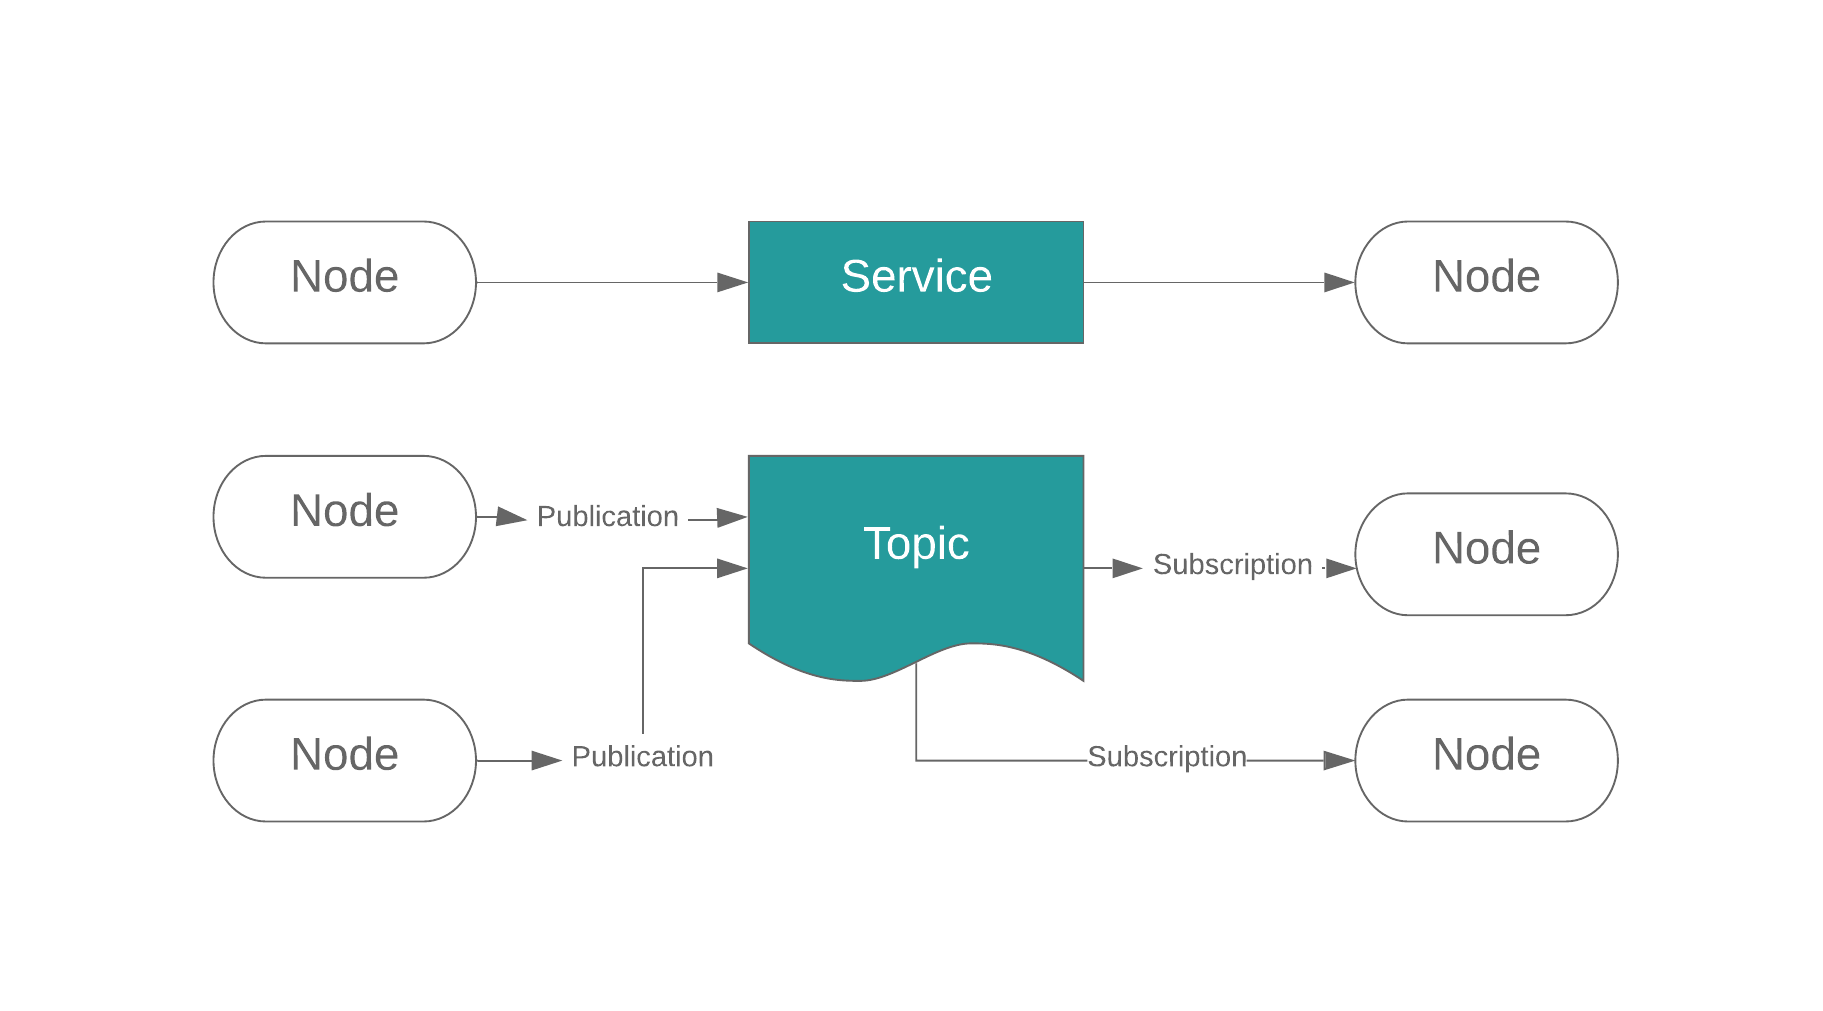
\includegraphics[width=1\textwidth]{images/Dada/RosNodesandTopics.png}%
     % you need to add the caption for the list of figures
    \caption[ROS Nodes and Topics]{ROS Nodes and Topics}\label{fig: ROS Nodes and Topics}%
  \end{figure}
  
\subsection{ROS Nodes, Topics, and Messages}
\hspace{2cm}ROS nodes are processes that usually does some computation and are able to
communicate with each other. Some examples for this experiment are one node responsible for the IMU data, another node responsible for the Gps data, and another node responsible for processing both sensor data. They can communicate through the use of topics. In order for nodes to communicate, a unique topic, service, or server name must be assigned by the node. Afterwards, any node in the system can publish or subscribe to that topic name. Publishing to a topic is similar to sending data to that topic name, while subscribing is similar to receiving the data. Each topic must be assigned a proper message structure, either custom built or one of the ROS messages. For example, there is an already built ROS message for IMU that contains linear acceleration, angular velocity, and orientation data. It is important to note that the node publishing and subscribing to the topic must use the same message structure.\cite{web040}

\section{Data Flow Abstraction}
\hspace{2cm}In this section we will illustrate the flow of the data inside the main device (Raspberry Pi), that resides and drives the robot. The flow of data inside the main controller is as shown in fig \ref{fig: Main Controller Data Flow Diagram}.
\subsection{Data Flow Diagram}
\hspace{2cm}The main controller consists of the following modules:
\begin{enumerate}
    \item Task handler Module 
    \item Classical Controller Module
    \item Obstacle Avoidance Module
    \item Main controller Module
    \item Serial Communication Module
\end{enumerate}
\subsubsection{Task Handler Module }
\hspace{2cm}The Task handler module is a ROS node that contains a web server. The server receives the incoming HTTP POST requests, which contains the task data, Processing the data and generating a sequence of sub-tasks, each sub-task contains a position and a flag that defines if the classical controller or the Module should take control at that point, Finally publishing that task on a ROS topic.
\begin{figure}[H]%
    \center%
    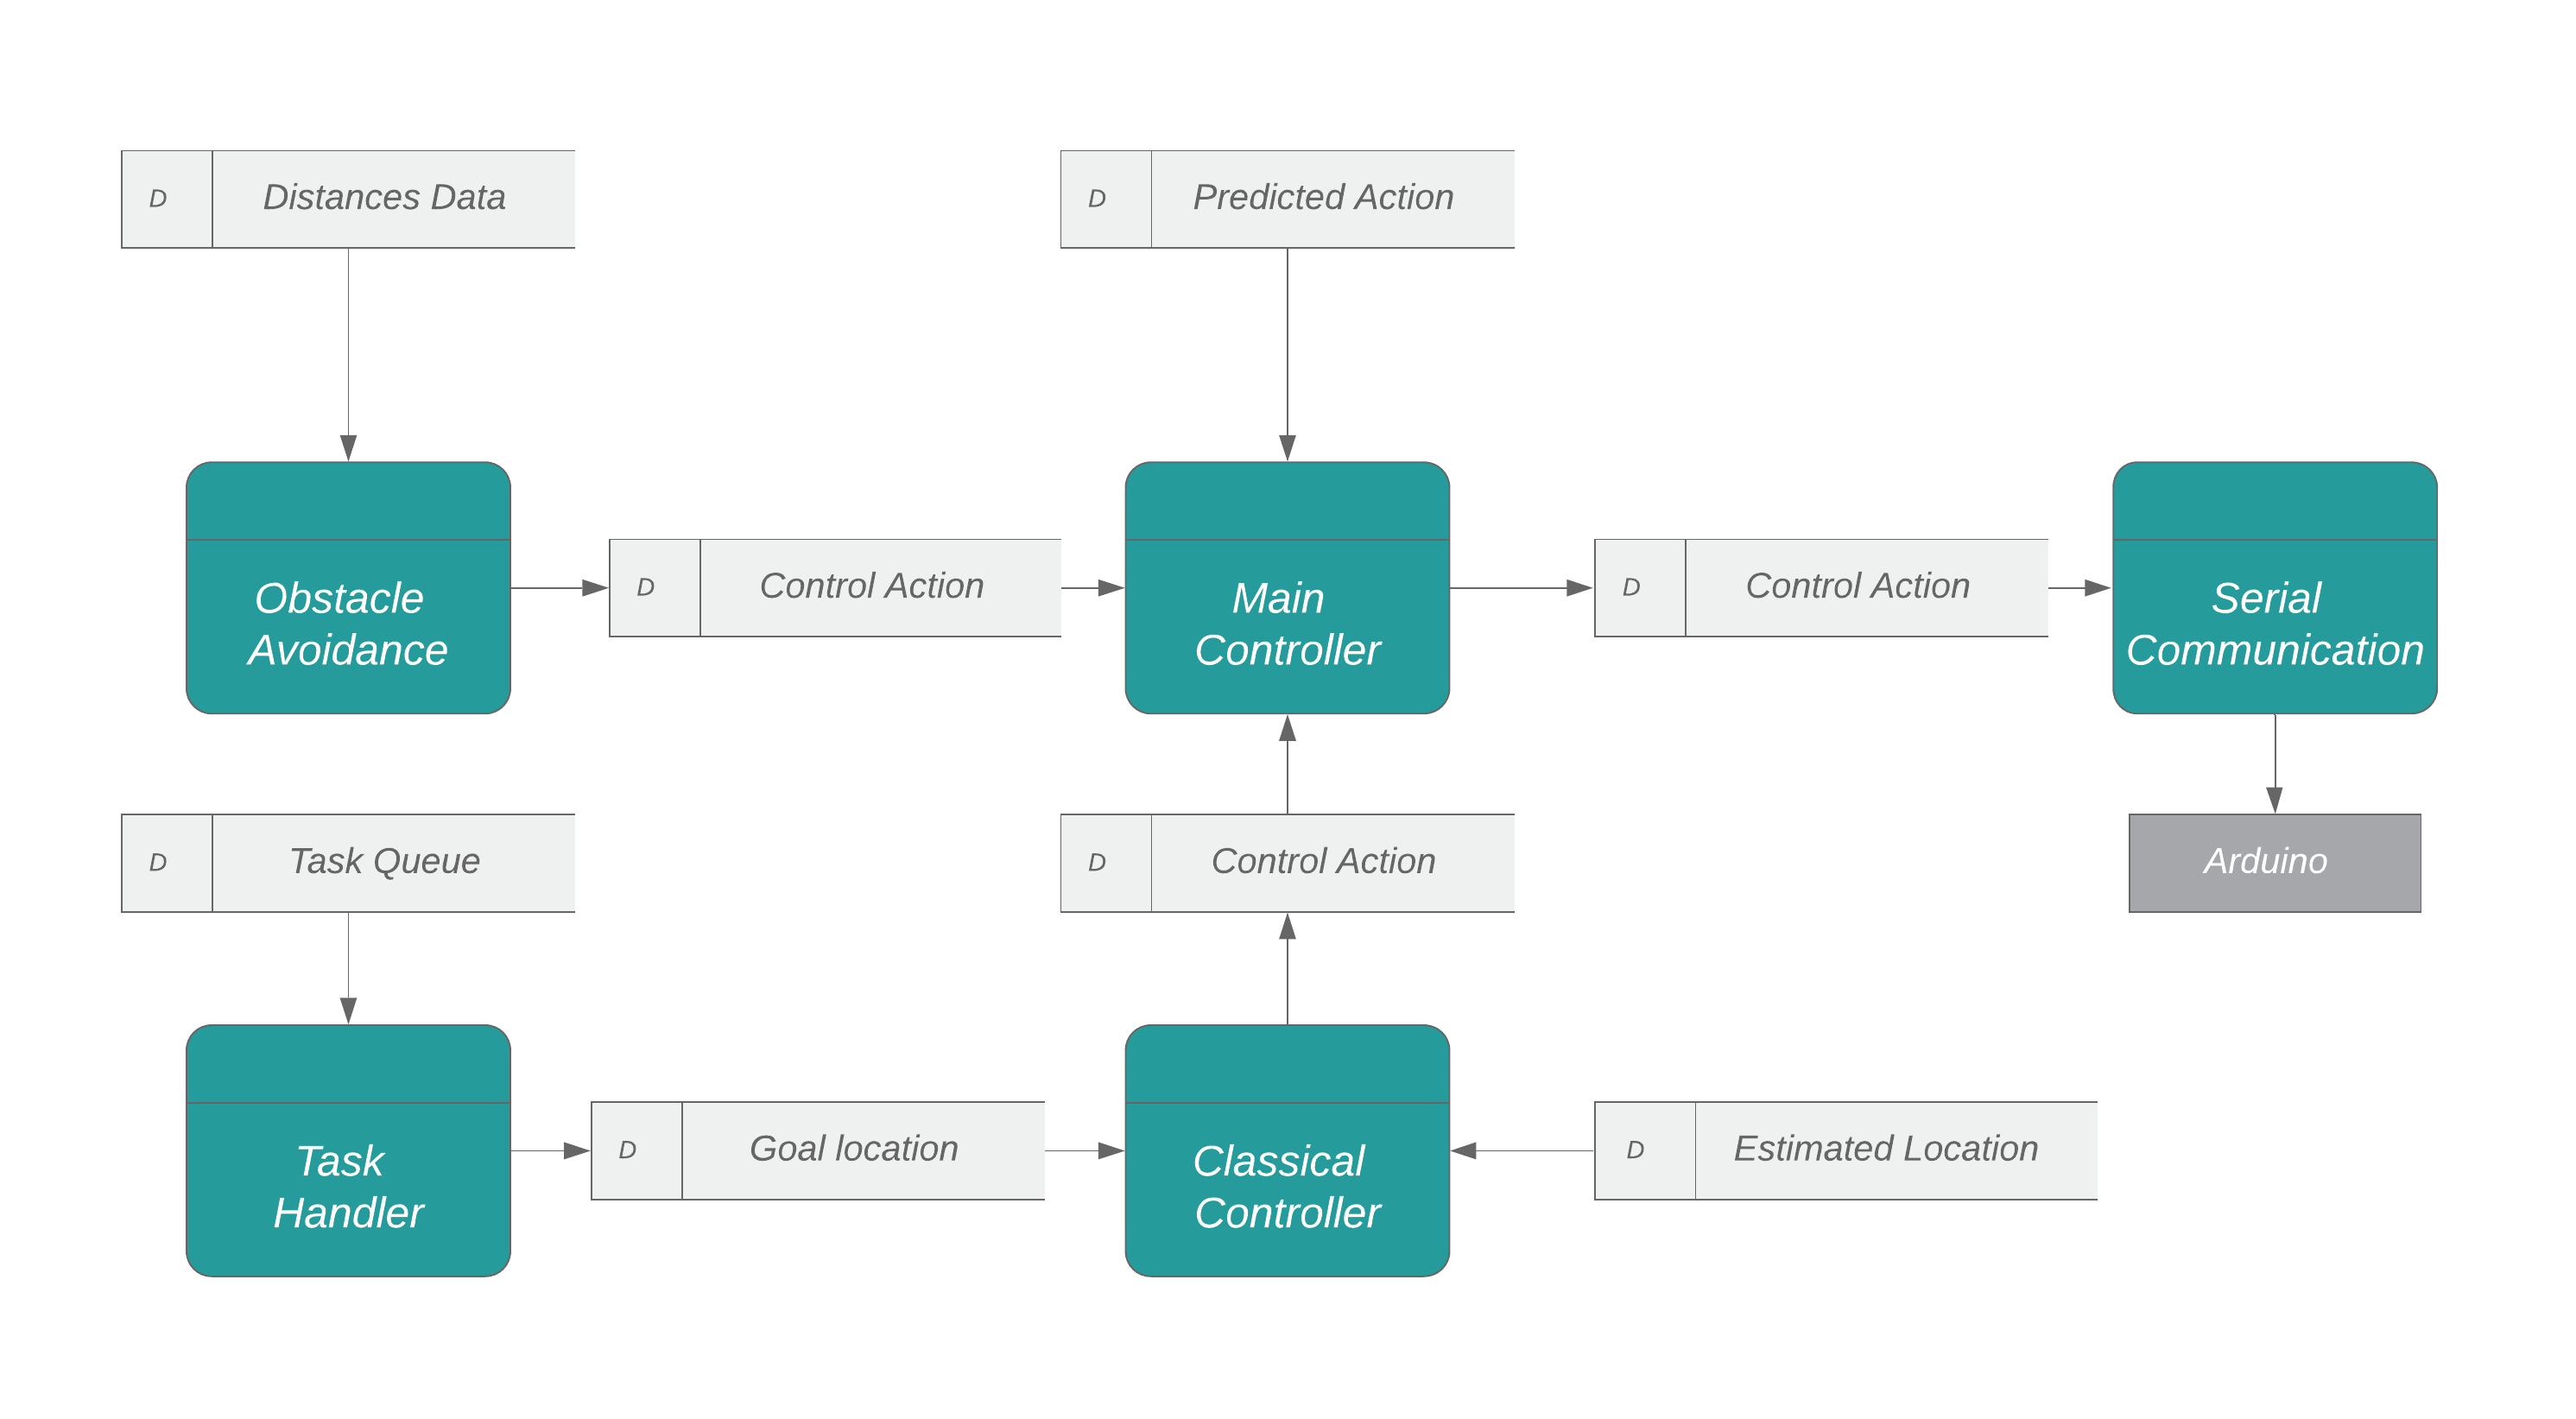
\includegraphics[width=.8\textwidth]{images/Dada/DataFlowDiagram.png}%
     % you need to add the caption for the list of figures
    \caption[Main Controller Data Flow Diagram]{Main Controller Data Flow Diagram}\label{fig: Main Controller Data Flow Diagram}%
  \end{figure}
\subsubsection{Classical Controller Module}
\hspace{2cm}The Classical Controller module is a ROS node, which takes the current location (estimated location from the localization module over a socket connection) and, the goal location ( provided from the task handler),  processing both location and generating the suitable control action to move the robot from the current location to the goal location
\subsubsection{Obstacle Avoidance Module}
\hspace{2cm}The Obstacle Avoidance module is a ROS node, which subscribes to the LIDAR data topic containing ranges and distances, then if the distance is below a certain threshold it outputs a high-priority control action, that is sent to the main controller.
\subsubsection{Main Controller Module}
 \hspace{2cm}The main controller is a ROS node that takes in all the control actions from the    Module, the obstacle avoidance module and the classical controller and based on the current information provided from the task handler, chooses which control action is sent to the serial communication module.
\subsubsection{Serial Communication Module}
\hspace{2cm}The Serial Communication module is a ROS Node that subscribes to the control action topic published from the main controller and then send it to the Arduino using serial port communication.

\section{Robot Work Environment}
\hspace{2cm}In this section we describe the main device environment on the robot. This main device communicates with the various components of the robot, after processing the data collected from them, it sends the appropriate control action to drive the actuators through the Arduino. We used The Nvidia Jetson TX1 development kit as our main computer, mainly because of it's computation capability, but due to some technical issues we were forced to downgrade to The Rasbpery pi model 3. The full hardware specification of the Rasbperry pi we used are on chapter 2.

\subsection{Raspberry Pi}
\hspace{2cm}In chapter 2 we covered the hardware specification of the Raspberry Pi we are using, we now introduce our work environment on the Raspberry Pi. We are using ROSbots \cite{web024}, which is Raspbian Stretch lite (Debian-based computer operating system for Raspberry Pi provided by the Raspberry Pi Foundation\cite{web025}) equipped with ROS Kinetic\cite{web026} and OpenCV  pre-installed on it.

\subsection{Operating ROS on The Raspberry Pi}
\hspace{2cm}The ROS Environment or ROS Work-space (as in ROS terms) on the Raspberry Pi consists of four essential packages:

\subsubsection{Sensors Package}
\hspace{2cm}Data acquisition package, It collects data from the sensors and, publishes each sensor's data to it's corresponding ROS Topic, So it could be used by other Nodes by subscribing to that topic.
\begin{enumerate}
    \item \textbf{IMU Node}\newline
        ROS Publisher Node that collects IMU data: Linear velocity and angular orientation and publishes this data on the IMU topic.
    \item \textbf{GPS Node}\newline
        ROS Publisher Node that collects GPS data: Longitude and latitude and, publishes this data on the GPS topic.
    \item \textbf{Camera Node}\newline
        ROS Publisher Node that collects Camera data: raw images and publishes this data on the Camera topic.
\end{enumerate}

\subsubsection{Control Package}
\hspace{2cm}The Control package is mainly used to generate control action that is published to the control action topic, whether it's generated while driving the robot manually or, while the robot is being driven autonomously by the NN model.
\begin{enumerate}
    \item \textbf{Keyboard Node}\newline
    ROS Publisher Node that generates control action in response  to the keys being pressed by the keyboard while manually driving the robot to collect data for model training.
    \item \textbf{Autopilot Node}\newline
    ROS Publisher Node that subscribes to the Camera Topic, pass the image through the NN model, Then publishing the predicted control action on the control action topic.
\end{enumerate}

\subsubsection{Communication Package}
\hspace{2cm}Communication Package contains nodes that send data from the main device to other devices or modules of the system. Through serial port communication with the Arduino, or Socket connection with the localization module.
\begin{enumerate}
    \item \textbf{Serial Node}\newline
        ROS Listener Node that subscribes to the control action topic, Continuously sending the control action to the Arduino Uno over an open serial port communication.
    \item \textbf{Data Collector Node}\newline
        ROS Listener Node that subscribes to both camera and control action topics, store both of them in an object-like data, then saves the collected data to the hard disk to be used for NN model training later.
    \item \textbf{Socket Server Node}\newline
        ROS Listener Node that subscribes to sensors topics: IMU and GPS, also the control action topic, then send them to the Localization module (socket client) through open server-client socket connection.
\end{enumerate}

\subsubsection{Web Server Package}
\hspace{2cm}Web Server Package is considered to be the bridge between the main system's web server and the ROS environment on the robot.

\begin{enumerate}
    \item \textbf{Task Handler Node}\newline
    ROS Publisher Node that contains a python web server, Capable of Handling the incoming HTTP requests that contain the task's data, Processing that data and publishing it to the task topic.
\end{enumerate}
%%%%%%%%%%%%%%%%%%%%%%%%%%%%%%%%%%%%%%%%%%%%%%%%%%%%%%%%%%%%%%%%%%%%%%%%%%%%%%%%%%%%%%%%%%%%%%%%%%%%%%%%%%%%%%%%%%
     \cleardoublepage%
     
     %%%%%%%%%%%%%%%%%%%%%%%%%%%%
% CHAPTER                  %
%%%%%%%%%%%%%%%%%%%%%%%%%%%%
\chapter{Robot Model and Motion Control}%
\label{chap:chap4}

%%%%%%%%%%%%%%%%%%%%%%%%%%%%
% SECTION                  %
%%%%%%%%%%%%%%%%%%%%%%%%%%%%
\newline
\newline
\vspace{3mm}
\hfill

\section{Introduction}
\hspace{2cm}In this chapter we discuss the model of our mobile robot and the low level motion control. As mentioned before our Wild Thumper is a differential drive model that takes linear and angular velocities as input, (which is different from a car-like model that takes  linear velocity and  steering angle as input). To have an appropriate and stable motion for the required velocities, low-level motion control is used to control the motion of the robot depending on the kinematics discussed below and the drivers. \\

\section{Differential Drive Robot}
\hspace{2cm}Differential Drive Robot is the simplest drive mechanism which controlled through left and right velocities (low level motion control) to move from a starting point to a global goal passing through some local goals, which called Robot Locomotion. Robot Locomotion is a mechanism of motion that describes the methods robots use to be transported from one location to another. \\
In figure \ref{fig: diff drive} , differential drive robot (is most common in two wheeled robots) has $v_r$ and $v_l$ parameters (right and left velocities respectively) which control the robot’s motion, and $R$ parameter which stands for Radius of curvature, it has two cases: \\
- The first case: Radius can be infinite, thus the angular velocity is zero resulting in a linear motion only, according to formula: $v = w * R$ \\
- The second case: If the $R$ parameter has a value which means that the robot has an angular velocity that will produce a rotation around ICR (Instantaneous Center of Rotation).\\

\begin{figure}[H]%
    \center%
    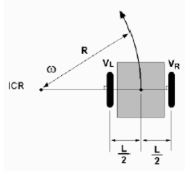
\includegraphics[width=.5\textwidth]{images/Alzahraa/differential_drive.JPG}%
     % you need to add the caption for the list of figures
    \caption[Differential Drive Robot]{The differential drive robot and its parameters}\label{fig: diff drive}%
  \end{figure}
  
%%%%%%%%%%%\figure number %%%%%%%%%%%%%%%%
Kinematics is geometric description of mechanical behavior of the robot for design and control.\cite{web001} 
The differential drive robot kinematics (forward and inverse kinematics), used in the control loop to follow the trajectory, as shown in figure \ref{fig: control loop}.

\begin{figure}[H]%
    \center%
    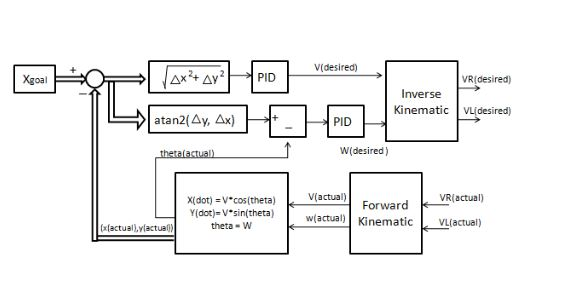
\includegraphics[width=.8\textwidth]{images/Alzahraa/control_loop.JPG}%
     % you need to add the caption for the list of figures
    \caption[Control Loop]{The control loop of differential drive robot}\label{fig: control loop}%
  \end{figure}
 
\subsection{Robot Forward kinematics}
\hspace{2cm}For differential drive robot, the linear and angular velocities are calculated using forward kinematics.
At each time instant, the right and left wheels must follow a trajectory that moves around the ICR at the same angular rate:
\begin{align*}
w(R + \frac{L}{2}) & = v_r  &  w(R - \frac{L}{2}) & = v_l
\end{align*}
 Where $L$  is the distance between any two facing wheels,$v$ is the linear velocity and $w$ is the angular velocity.
From these two equations and the formula: $v = w * R$ , the linear and angular velocities are calculated using the following equations:
\begin{align*}
v & = \frac{v_r + v_l}{2} & w & = \frac{v_r - v_l}{2}
\end{align*}
\subsection{Robot Inverse kinematics}
\hspace{2cm}Practically, to follow a specified trajectory given a new goal to be achieved described by ($x$,$y$,\(\theta)\) and the suitable values for $v$ and $w$, the required will be right and left velocities which are calculated using inverse kinematics according to the following equations:
\begin{align*}
v_r & = v + \frac{w * L}{2} & v_l & = v - \frac{w*L}{2}
\end{align*}
%
%\section{Serial communication}
%The Values of linear and angular velocities are determined by high level controller to achieve the desired goal, these values are calculated on a computer device which in our case is Nvidia Jetson Tx1 and then they are sent to Arduino using serial communication.
%sSerial is used for communication between the Arduino board and a computer or other devices. All Arduino boards have at least one serial port (also known as a UART or USART): Serial. It communicates on digital pins 0 (RX) and 1 (TX) as well as with the computer via USB. And by using Serial.read( ) function in Arduino that reads the incoming serial data, the values of both v and w is ready to be applied.\cite{web002}

\section{Low-level Motion Control}
\hspace{2cm} Control is divided into two levels, a low-level that receives $v$ and $w$ and applies the suitable voltages to motors, and a higher-level that determines the values of $v$ and $w$.
\subsection{Motor Drivers}
\hspace{2cm}Motor Driver circuits are current amplifiers. They act as a bridge between the controller and the motor in a motor drive. Motor drivers are made from discrete components which are integrated inside an IC. The input to the motor driver IC or motor driver circuit is a low current signal. The function of the circuit is to convert the low current signal to a high current signal. This high current signal is then given to the motor which helps to drive it.\cite{web003}
In robotics, To drive the robot in two opposite directions: forward and backward, H bridge is used to run the motor based on IN1 and IN2 values which are signals received from arduino and fed to the motor driver as shown in figure \ref{fig: transistor} and figure \ref{fig:possible cases}.\\
And to control the speed of DC motors, pulse width modulation pins of Arduino controller is used.
\begin{figure}[H]%
    \center%
    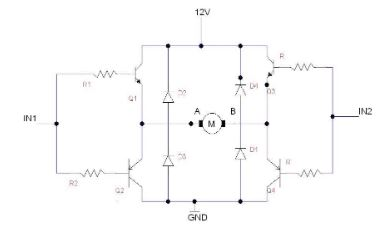
\includegraphics[width=.8\textwidth]{images/Alzahraa/H_bridge.JPG}%
     % you need to add the caption for the list of figures
    \caption[Transistor H-bridge]{Transistor Based H-Bridge Circuit\cite{web003}}\label{fig: transistor}%
  \end{figure} 
  \begin{figure}[H]%
    \center%
    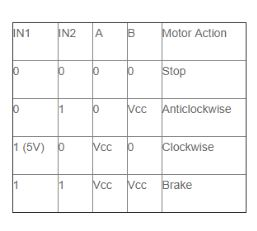
\includegraphics[width=.8\textwidth]{images/Alzahraa/possible_cases.JPG}%
     % you need to add the caption for the list of figures
    \caption[Possible Cases of Motor Driver Pins]{The four possible cases of IN1 and IN2 \cite{web003}}\label{fig:possible cases}%
  \end{figure} 
\subsection{Pulse Width Modulation}
\hspace{2cm}PWM is used to produce Analog signals from a digital device like an Arduino, to control the speed of the motors.\\
PWM signal’s values are varying from  0 to 255, 255 is the largest value that drives the motor by the maximum speed and 0 will result in stopping the motor. 
We can determine how long the motor is on and how long the motor is off according to the duty cycle percent, so if the duty cycle is 100\% this means it is fully on and if the duty cycle is 50\% this means a digital signal is on half of the time and off for the other half of the time and so on. Illustrated in figure \ref{fig:pwm} 
  \begin{figure}[H]%
    \center%
    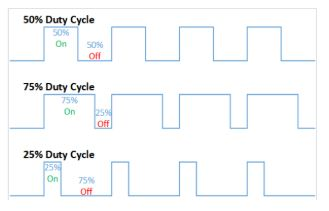
\includegraphics[width=.8\textwidth]{images/Alzahraa/duty_cycle.JPG}%
     % you need to add the caption for the list of figures
    \caption[Pulse Width Modulation]{Three scenarios of the duty cycle}\label{fig:pwm}%
  \end{figure} 
To achieve the required PWM value we map the desired voltage to its corresponding PWM signal using this relation:  \(pwm =  \frac{volt}{maximumVolt} * 255 \) then it can applied directly to the motor.

\subsection{Motors Calibration}
\hspace{2cm}Calibration is the setting or correcting of a measuring device or base level, usually by adjusting it to match or confirm to a dependably known and unvarying measure.\cite{web004}\\
In our project we calibrated the linear velocity to its corresponding value of voltage. So that for each required linear velocity, the suitable voltage will be applied. The angular velocity is calibrated from desired to actual values due to frictional force.\\
\subsubsection{Robot Linear Velocity Calibration}
\hspace{2cm}The robot is driven by Arduino code with known and equal PWM  on both sides of the robot and respectively known voltages, it moves linearly for a distance that is measured in meters and known time that is measured in seconds by a stopwatch. By using the velocity formula: \(v = \frac{s}{t}\)  linear velocities can be calculated for many values of PWM that are shown in Table \ref{table:linear_calibration}. And a polynomial function that relates the velocities to voltages can be described as:\\
For right side motors: \(V=0.2042 v^2+6.2299 v+0.4462 \)
And for left side motors: \(V=0.2047 v^2+6.2452 v+0.4473\)
The plot diagram that shows the relation between the velocity and the voltage which is limited within the recommended voltages (2-7.5) is represented in figure \ref{fig:linear calibration}
 
\begin{table}[h!]
\centering
\begin{tabular}{|c|c|c|c|c|} 
 \hline
 \multicolumn{5}{| c |}{Right Motors}\\
 \hline
 \hline
 PWM & Voltage (volts) & Distance (meters) & Time (seconds) & Velocity (m/s) \\ [0.5ex] 
 \hline\hline
 
23& 0.736& 0& 0& 0\\
30& 0.96& 2.84& 26.13& 0.1086\\
40& 1.28& 2.84& 18.49& 0.1535\\
60& 1.92& 2.84& 11.36& 0.25\\
80& 2.56& 2.84& 8.3& 0.3421\\
100& 3.2& 2.84& 6.54& 0.4342\\
120& 3.84& 2.84& 5.49& 0.5173\\
140& 4.48& 2.84& 4.19& 0.6778\\
160& 5.12& 2.84& 3.8& 0.7473\\
180& 5.76& 2.84& 3.47& 0.8184\\
200& 6.4& 2.84& 3.35& 0.8477\\
220& 7.04& 2.84& 2.75& 1.0327\\
240& 7.68& 2.84& 2.5& 1.136\\
255& 8.16& 2.84& 2.37& 1.1983 \\[1ex] 
 \hline
\end{tabular}
\end{table}

\begin{table}[h!]
\centering
\begin{tabular}{|c|c|c|c|c|}
 \hline
 \multicolumn{5}{| c |}{Left Motors}\\
 \hline
 \hline
 PWM & Voltage (volts) & Distance (meters) & Time (seconds) & Velocity (m/s) \\ [0.5ex] 
 \hline\hline
 
23& 0.7378& 0& 0& 0\\
30& 0.9623& 2.84& 26.13& 0.1086\\
40& 1.2831& 2.84& 18.49& 0.1535\\
60& 1.9247& 2.84& 11.36& 0.25\\
80& 2.5662& 2.84& 8.3& 0.3421\\
100& 3.2078& 2.84& 6.54& 0.4342\\
120& 3.8494& 2.84& 5.49& 0.5173\\
140& 4.4909& 2.84& 4.19& 0.6778\\
160& 5.1325& 2.84& 3.8& 0.7473\\
180& 5.7741& 2.84& 3.47& 0.8184\\
200& 6.4156& 2.84& 3.35& 0.8477\\
220& 7.0572& 2.84& 2.75& 1.0327\\
240& 7.6988& 2.84& 2.5& 1.136\\
255& 8.18& 2.84& 2.37& 1.1983\\[1ex] 
 \hline
\end{tabular}
\caption[Robot Linear Velocity Calibration]{Robot linear velocity calibration}
\label{table:linear_calibration}
\end{table}

\clearpage


  \begin{figure}[H]%
    \center%
    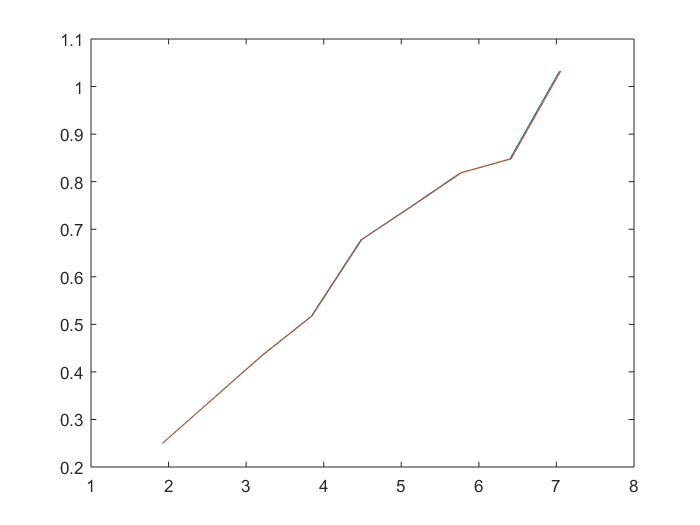
\includegraphics[width=.8\textwidth]
    {images/Alzahraa/linear_calibration.jpg}%
     % you need to add the caption for the list of figures
    \caption[Robot Linear Velocity Calibration]{The relationship between the velocity as a vertical axis and the voltage as a horizontal axis within recommended voltages}\label{fig:linear calibration}%
  \end{figure} 
  
\subsubsection{Robot Angular Velocity Calibration}
\hspace{2cm}Due to frictional force, the desired angular velocity can not be achieved by applying the right and left velocities calculated from inverse kinematics. Therefore a calibration between the desired and the actual angular velocities is required. By applying zero linear velocity with many values of angular velocities and measuring the actual for each one as shown in Table \ref{table:angular_calibration}, The relation between desired and actual angular velocities is described as: \(actual =  2 * desired + 0.55\)
\begin{table}[h!]
\centering
\begin{tabular}{|c|c|}
 \hline
 Desired Angular Velocity (rad/s) &Actual Angular Velocity (rad/s)\\ [0.5ex] 
 \hline\hline
 
0.785 & 2\\
1.57 & 3.8\\
2.355 & 5.1\\
3.14 & 6.7\\
[1ex] 
 \hline
\end{tabular}
\caption[Robot Angular Velocity Calibration]{Robot angular velocity calibration}
\label{table:angular_calibration}
\end{table}

\section{Arduino Applied Code Flow}
\hspace{2cm}The low level motion sequence is starting be receiving desired linear and angular velocities from high level controller, then apply inverse kinematic to calculate the desired right and left velocities. Then to be applied to the motors these velocities mapped to their corresponding voltages according to the previous calibration equations which finally mapped to their corresponding PWM values.\\
To recap this sequence we can consider the flowchart represented in figure \ref{fig:arduino_code}:

  \begin{figure}[H]%
    \center%
    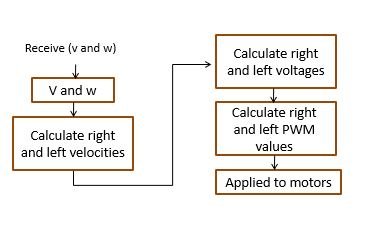
\includegraphics[width=.8\textwidth]{images/Alzahraa/flowchart.JPG}%
     % you need to add the caption for the list of figures
    \caption[Arduino Applied Code Flow]{}\label{fig:arduino_code}%
  \end{figure} 
%%%%%%%%%%%%%%%%%%%%%%%%%%%%%%%%%%%%%%%%%%%%%%%%%%%%%%%%%%%%%%%%%%%%%%%%%%%%%%%%%%%%%%%%%%%%%%%%%%%%%%%%%%%%%%%%%%
     \cleardoublepage%
    
     %%%%%%%%%%%%%%%%%%%%%%%%%%%%
% CHAPTER                  %
%%%%%%%%%%%%%%%%%%%%%%%%%%%%
\chapter{Motion Planning and Navigation}%
\label{chap:chap5}

%%%%%%%%%%%%%%%%%%%%%%%%%%%%
% SECTION                  %
%%%%%%%%%%%%%%%%%%%%%%%%%%%%
\newline
\newline
\vspace{3mm}
\hfill
\section{Introduction}
\hspace{2cm} In this chapter we present an overview of the whole system components, their architecture, usage and how they are connected. We also present system modules that perform the functionality of the system and how they are integrated together. And a business scenario that recaps the flow of the project.
\section{Long-term Planning}
\hspace{2cm}Map based planning responsible for generating a path from start to the Goal.

\subsection{Path Planning Algorithm}
\hspace{2cm}The key to achieve the best path between points A and B, as we know from everyday life, is to use a map. Typically, best means the shortest distance but it may also include some penalty term or cost related to traversability which is how easy the terrain is to drive over – it might be quicker to travel further but over better roads. A more sophisticated planner might also consider the kinematics and dynamics of the vehicle and avoid paths that involve turns that are tighter than the vehicle can execute. A robot may be defined as: \textbf{“A goal oriented machine that can sense, plan and act”} This section concentrates on planning.
There are many ways to represent a map and the position of the vehicle within the map. One approach is to represent the vehicle position as $(x, y) \in R^2$ and the derivable regions or obstacles as polygons, each comprising lists of vertices or edges. This is potentially a very compact format but determining potential collisions between the robot and obstacles may involve testing against long lists of edges. A simpler and very computer-friendly representation is graph. As it consists of nodes and edges and it will be discussed below.

\subsection{Path Planning Algorithm Assumptions}
\hspace{2cm}We state some assumptions for the algorithm.
Firstly, the robot operates in a graph world, graph consists of nodes which represent each intersection and edges which represent the roads as shown in figure  \ref{fig: Map} . 
Secondly, the robot can move to only neighbors on the same direction of its bearing. 
Thirdly, the start and the goal may not on existing node in our graph so to handle this case, we add the start and the end as new node and find its position on the graph by finding the Equation between each node and this node will be located on the edge that achieve the equation.
Fourthly, there are many roads that consist of two lanes in the same direction, may be one of them is closer to goal than the other, so to find the best and shortest path to goal we assume that there are two nodes which represent the start of the two lanes and also there are two nodes which represent the goal from two direction.

\begin{figure}%
    \center%
    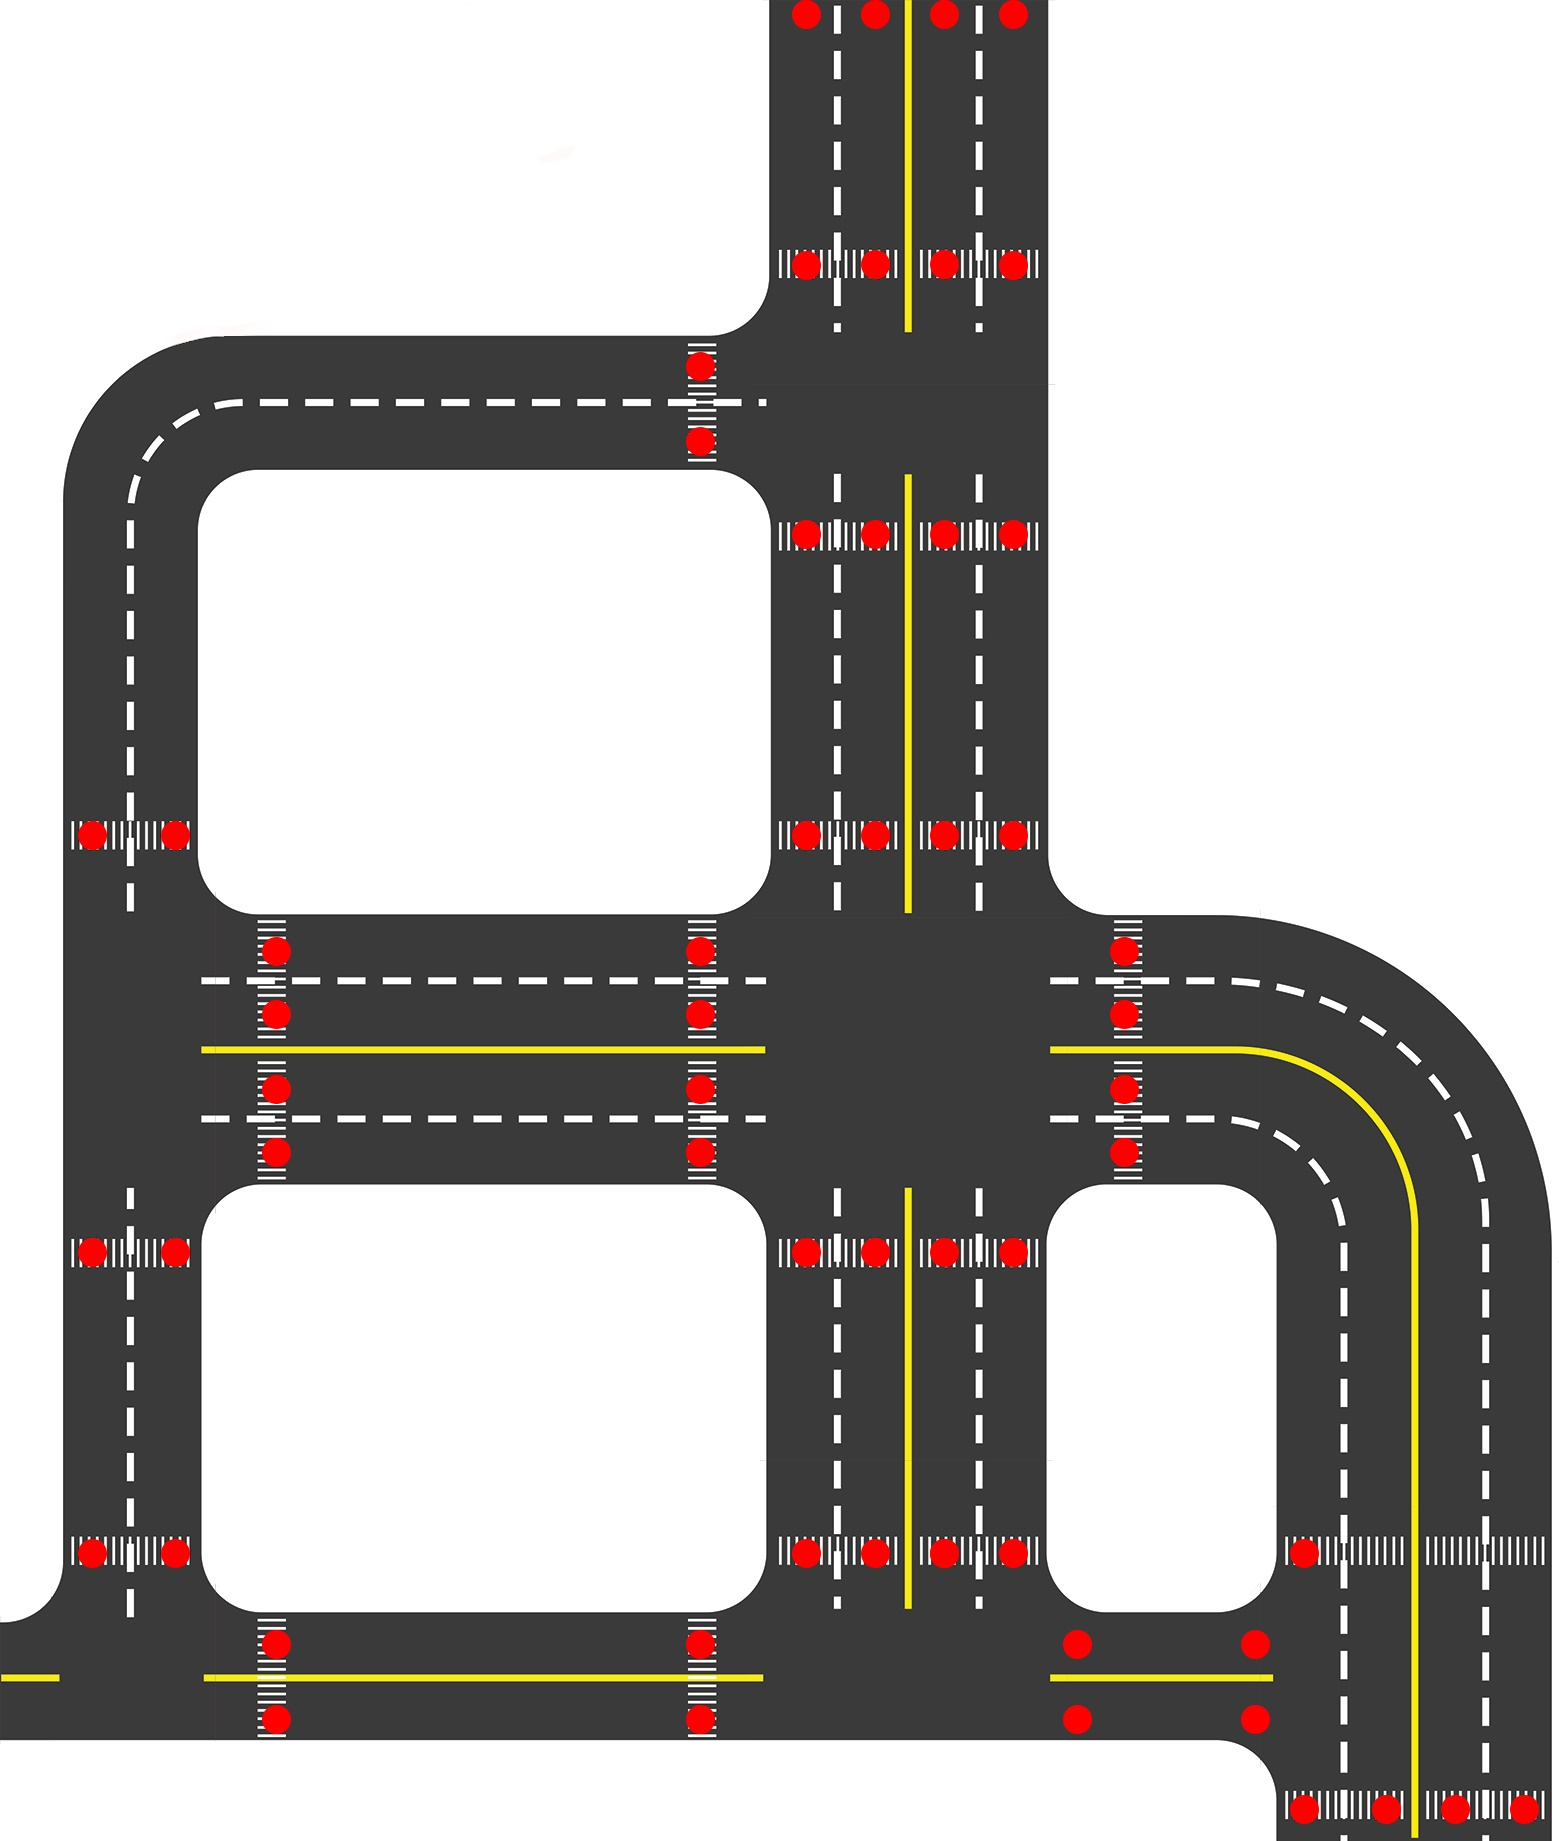
\includegraphics[width=1\textwidth]{images/motion/map.jpg}%
     % you need to add the caption for the list of figures
    \caption[Map]{Map}\label{fig: Map}%
  \end{figure}

\subsection{A* Algorithm}
\hspace{2cm}A* is a path finding algorithm that can be used to find the shortest path from the current location of the robot to the goal location.
A* uses a best-first search and finds a least-cost path from the given initial current location to the goal location. As A* traverses the map, it follows a path of the lowest expected total cost or distance, keeping a sorted priority queue of alternate path segments along the way. It uses a knowledge-plus-heuristic cost function of cell x (usually denoted f(x)) to determine the order in which the search visits adjacent cells in the map. The cost function is a sum of two functions: - the past path-cost function, which is the known distance from the starting node to the current node x (usually denoted g(x)) - a future path-cost function, which is an admissible "heuristic estimate" of the distance from x to the goal (usually denoted h(x)). The h(x) part of the f(x) function must be an admissible heuristic; that is, it must not overestimate the distance to the goal. Thus, for our application, h(x) might represent the straight-line distance to the goal, since that is physically the smallest possible distance between any two cells. \newline

Like all informed search algorithms, it first searches the routes that appear to be most likely to lead towards the goal. What sets A* apart from a greedy best-first search is that it also takes the distance already traveled into account; the g(x) part of the heuristic is the cost from the starting point, not simply the local cost from the previously expanded cell. Starting with the initial cell, it maintains a priority queue of cells to be traversed, known as the open set or fringe. The lower f(x) for a given cell x, the higher its priority. At each step of the algorithm, the cell with the lowest f(x) value is removed from the queue, the f and g values of its neighbors are updated accordingly, and these neighbors are added to the queue. The algorithm continues until a goal cell has a lower f value than any cell in the queue (or until the queue is empty). The f value of the goal is then the length of the shortest path, since h at the goal is zero in an admissible heuristic. \newline

The algorithm described so far gives us only the length of the shortest path. To find the actual sequence of steps, the algorithm can be easily revised so that each node on the path keeps track of its predecessor. After this algorithm is run, the ending node will point to its predecessor, and so on, until some node's predecessor is the start node.

\subsection{Graph-based Path Planning}
\hspace{2cm}In this part we introduce our approach to the path planning problem. We start with the method we used to represent and store our world's map, Then we define the method we used to extract useful information out of the graph's data, Data like the cost and edge equations, Finally we provide a pseudo-code of the modified A * algorithm we used.
\subsubsection{Map Input}
This file used to enter all data about each node in the graph. the output is file that contain graph map.
this data are :
 \begin{enumerate}
    \setcounter{enumi}{0}
    \item Node Name.
    \item Position or the Coordinates of the node.
    \item Children of the node.
    \item Parent of The node.
    \item Node direction
    \item Children of this node
    \item  if a decision has been token or not.
    \end{enumerate}
\subsubsection{Map Calculations}
We now have our world's map stored as a file, containing all the nodes with all of their data, Now we input that file to the map calculations script, which does the following:
\begin{enumerate}
    \item Reads in the graph file from the hard disk and store the graph data to a suitable data structure.
    \item For each node in the graph, Calculate the distance (which is later used as the cost as discussed in the A * section) between that node and all their children nodes
    \item For each node in the graph, calculate the Linear equation between that node and all its children. These equations are used later for edge detection, when we add new nodes to the graph
    \item Adding the calculated distances and edge equations to the data structure and then rewrite them to disk for storing.
\end{enumerate}
\subsubsection{A * Pseudocode}
\begin{enumerate}
    \setcounter{enumi}{0}
        \item we assume that we have two lists: 
            \begin{itemize}
            \item Open list that is set of tentative nodes to be evaluated, initially containing the start node.
            \item closed list contain nodes already evaluated.
            \end{itemize}
    \item  Add the starting node to the open list.
    \item Repeat the following:
        \begin{itemize}
        \item Look for the lowest F cost node on the open list. We refer to this as the current node.
        \item . Switch it to the closed list.
        \item  For each of the 8 squares adjacent to this current square:
            \begin{enumerate}
            \item If it is not walkable or if it is on the closed list, ignore it. Otherwise do the following.
            \item If it isn’t on the open list, add it to the open list. Make the current node the parent of this node. Record the F, G, and H costs of the node.
            
           \item If it is on the open list already, check to see if this path to that node is better, using G cost as the measure. A lower G cost means that this is a better path. If so, change the parent of the node to the current node, and recalculate the G and F scores of the square. If you are keeping your open list sorted by F score, you may need to resort the list to account for the change.
            \end{enumerate}
        \end{itemize}   
        \item Stop when you:
            
         \begin{enumerate}
            \item Add the target node to the closed list, in which case the path has been found, or
            \item Fail to find the target node, and the open list is empty. In this case, there is no path
            
           \item Save the path. Working backwards from the target node, go from each node to its parent node until you reach the starting node. That is your path.\cite{A-Star} 
            \end{enumerate}
\end{enumerate}
After the web server has finished processing the customer's order, Three point are sent to the Path planning Module:
\begin{enumerate}
    \item Robot Base location
    \item Vendor's Location
    \item Customer's Location
\end{enumerate}
Generating these Three paths:
\begin{enumerate}
    \item Base-Vendor path
    \item Vendor-Customer path
    \item Customer-Base Path
\end{enumerate}
These three paths are considered the task, that is sent to the robot.


    
    
    





\section{Short-term Planning}

\hspace{2cm} The path that will be followed by the robot is a sequence of nodes, the current node can be decision or non-decision node. Our main controller will decide according to the robot state what is the appropriate action the robot should take by switching between three modules, classical control, learning control and obstacle avoidance at appropriate time to help the robot to reach the final destination. We will discuss each module separately in this section.

\subsection{Classical Control}

\hspace{2cm} The classical control theory uses a mathematical model to define the relationships between the input and output of a system. The most common type of these controllers are PID controllers. After they take the output of the system and compare it with the desired input, they generate an appropriate control signal based on the calculated error value.\cite{classical_control} A PID controller (proportional–integral–derivative controller) used to calculate the error which represent the difference between the setpoint (desired value ) and the measured variable and applies the correction.

In our project, we use classical methods to control the robot at intersection points on the map as shown in figure \ref{fig:intersetion points}. 
   \begin{figure}[H]%
    \center%
    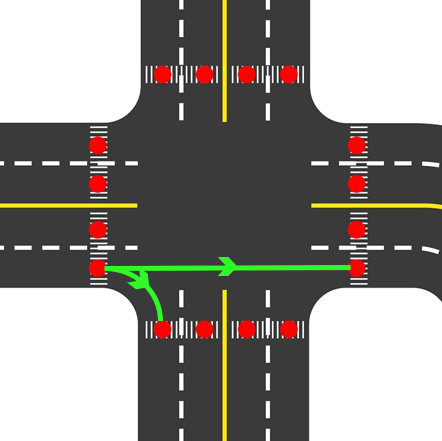
\includegraphics[width=.5\textwidth]
    {images/Alzahraa/intersectionPoints.png}%
    \caption[Map's Intersection Points]{Intersection points}\label{fig:intersetion points}%
  \end{figure}
  
With the help of state estimator that will be explained in section \ref{stateEstimator}, the current pose of the robot is determined and respectively the current node in path which tells if a decision has to be made at this node or not. If it is a decision node, the responsibility of controlling the robot is set to classical control.\\
The next node is retrieved from path and by calculating the distance between current and next node we can calculate the radius of curvature (R). \\
The linear velocity of the robot is constant and has the same value that is generated from the CNN model, so the required angular velocity to move the robot to the next node can be determined from this formula: $ w = v / R$.\\

\begin{figure}[H]%
    \center%
    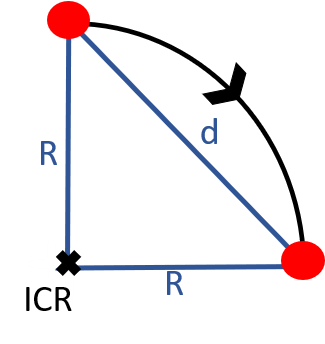
\includegraphics[width=.3\textwidth]
    {images/Alzahraa/classical.png}%
    \caption[Classical Control]{Determining value of angular velocity}\label{fig:w calculation}%
  \end{figure}

\subsection{Learning Control}
\hspace{2cm} imitation learning is considered one of the way of controlling autonomous cars that integrates prior driving experiences – a system that will help the cars perform on the road.
 car in the right

imitation learning can be used to train a convolutional neural network that maps perceptual inputs to
control commands; for example, mapping camera images to
velocity and the angle of velocity. This approach has been applied to lane following.
this will be discussed in section\ref{learn} .

\subsection{Obstacle Avoidance}
\hspace{2cm} In robotics, obstacle avoidance is the task of satisfying some control objective subject to non-intersection or non-collision position constraints. In unmanned air vehicles, it is a hot topic.What is critical about obstacle avoidance concept in this area is the growing need of usage of unmanned aerial vehicles in urban areas for especially military applications where it can be very useful in city wars. Normally obstacle avoidance is considered to be distinct from path planning in that one is usually implemented as a reactive control law while the other involves the pre-computation of an obstacle-free path which a controller will then guide a robot along. With recent advanced in the autonomous vehicles sector, a good and dependable obstacle avoidance feature of a driverless platform is also required to have a robust obstacle detection module.\cite{web038}

\par
In our project, we simply detect the obstacles by using LIDAR sensor only. LIDAR sensor gives the range between it and the obstacle and compare this range with a threshold to generate an appropriate linear and angular velocities that will help the robot to avoid this obstacle at appropriate time as shown in the figure below.
We used "testbot\_description" ROS Package to implement obstacle avoidance.
\par


 \begin{figure}[H]%
    \center%
    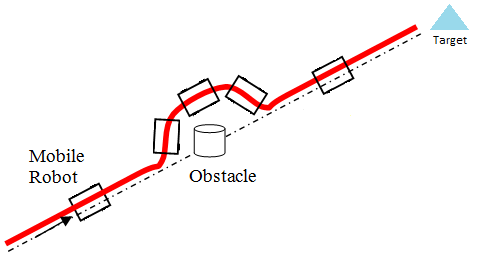
\includegraphics[width=.8\textwidth]{images/Alaa/Obstacle-avoidance.png}%
     % you need to add the caption for the list of figures
    \caption[obstacle avoidance]{The scenario of obstacle avoidance.}\label{fig: obstacle avoidance}%
  \end{figure}
 
\section{State Estimation for Robotics} \label{stateEstimator}

\hspace{2cm}A typical control system requires actual state measurement to perform the required task correctly. A robot pose represents its state for example. Due to sensor capabilities, measurement noise, and model uncertainty, it is not possible to know an actual state exactly. So, it is required to estimate system state from all uncertain  information about it. A state estimator is typically a computer implemented mathematical model and it provides the estimation of the internal states of the system. In most practical cases, the physical state of the system cannot be determined by direct observation. Instead, indirect effects of the internal state are observed by way of the system outputs.\cite{stateEstimator}
\par
We are using robot localization as state estimation, localization is the process of determining the position of the mobile robot by using sensor fusion concept. Sensor fusion is software that intelligently combines data from several sensors.\cite{web034}
\par
Using more sensors, increase the accuracy of localization algorithm (accurately locate the mobile robot) as shown in the figure below:


 \begin{figure}[H]%
    \center%
    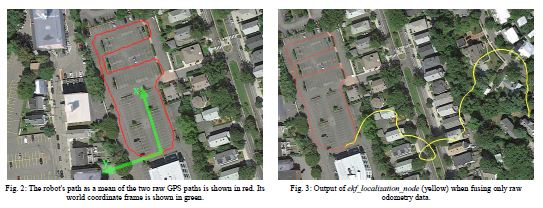
\includegraphics[width=.9\textwidth]{images/Alaa/sensorFusion0.JPG}%
  \end{figure}
  
 \begin{figure}[H]%
    \center%
    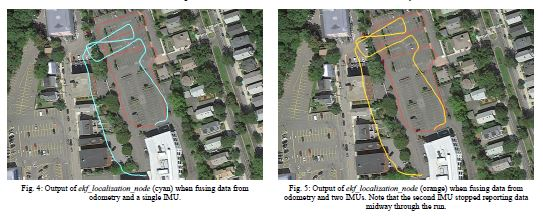
\includegraphics[width=.9\textwidth]{images/Alaa/sensorFusion1.JPG}%
  \end{figure}
  
   \begin{figure}[H]%
    \center%
    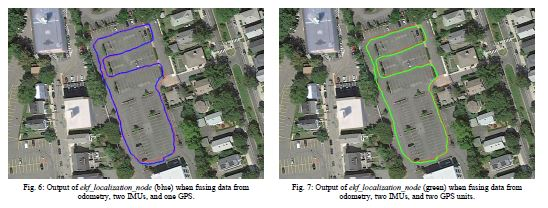
\includegraphics[width=.9\textwidth]{images/Alaa/sensorFusion2.JPG}%
     % you need to add the caption for the list of figures
    \caption[Sensor Fusion]{increasing number of sensors leads to increase the accuracy of locating the robot.}\cite{web035}\label{fig: Sensor Fusion}%
  \end{figure}
  
A stable and robust outdoor localization algorithm is critical to successful outdoor navigation. However, unpredictable external effects and interruption of the GPS signal cause difficulties in outdoor localization. So this is the reason of using multiple sensors on localization as we discussed previously in the so-called Sensor Fusion.
In our project we used the localization package integrated with ROS (robot\_pose\_ekf package).

\subsection {Extended Kalman Filter (EKF)}
\hspace{2cm} Most of the modern systems are equipped with numerous sensors that provide estimation of hidden (unknown) variables based on the series of measurements. For example, the GPS receiver provides the location and velocity estimation, where location and velocity are the hidden variables and differential time of satellite's signals arrival are the measurements.

One of the biggest challenges of tracking and control system is to provide accurate and precise estimation of the hidden variables in presence of uncertainty. In the GPS receiver, the measurements uncertainty depends on many external factors such as thermal noise, atmospheric effects, slight changes in satellite's positions, receiver clock precision and many more.

Kalman Filter is one of the most important and common estimation algorithms. The Kalman Filter produces estimates of hidden variables based on inaccurate and uncertain measurements. As well, the Kalman Filter provides a prediction of the future system state, based on the past estimations.

The filter is named after Rudolf E. Kalman (May 19, 1930 – July 2, 2016). In 1960, Kalman published his famous paper describing a recursive solution to the discrete-data linear filtering problem. \cite{kalmanFilter}\\

In our project we used extended Kalman filter (EKF) which is the nonlinear version of the Kalman filter that linearizes about an estimate of the current mean and covariance. In the extended Kalman filter, the state transition and observation models don't need to be linear functions of the state but may instead be differentiable functions:\\
     ${\displaystyle {\boldsymbol {x}}_{k}=f({\boldsymbol {x}}_{k-1},{\boldsymbol {u}}_{k})+{\boldsymbol {w}}_{k}} \\
   {\displaystyle {\boldsymbol {z}}_{k}=h({\boldsymbol {x}}_{k})+{\boldsymbol {v}}_{k}} \\ $
Here $w_k$ and $v_k$ are the process and observation noises which are both assumed to be zero mean multivariate Gaussian noises with covariance $Q_k$ and $R_k$ respectively. $u_k$ is the control vector.
The function $f$ can be used to compute the predicted state from the previous estimate and similarly the function $h$ can be used to compute the predicted measurement from the predicted state. However, $f$ and $h$ cannot be applied to the covariance directly. Instead a matrix of partial derivatives (the Jacobian) is computed.\\
At each time step, the Jacobian is evaluated with current predicted states. These matrices can be used in the Kalman filter equations. This process essentially linearizes the non-linear function around the current estimate.\cite{extendedKalmanFilter}\\
\textbf{Discrete-time predict and update equations:}\\
Notation  ${\displaystyle {\hat {\mathbf {x} }}_{n\mid m}} $represents the estimate of ${\displaystyle \mathbf {x} }$ at time $n$ given observations up to and including at time $m \leq n$. \\
\textbf{Predict}\\
Predicted state estimate:  	 ${\displaystyle {\hat {\boldsymbol {x}}}_{k|k-1}=f({\hat {\boldsymbol {x}}}_{k-1|k-1},{\boldsymbol {u}}_{k})}$ \\
Predicted covariance estimate: ${\displaystyle {\boldsymbol {P}}_{k|k-1}={{\boldsymbol {F}}_{k}}{\boldsymbol {P}}_{k-1|k-1}{{\boldsymbol {F}}_{k}^{\top }}+{\boldsymbol {Q}}_{k}}$ \\
\textbf{Update}\\
Innovation or measurement residual: ${\displaystyle {\tilde {\boldsymbol {y}}}_{k}={\boldsymbol {z}}_{k}-h({\hat {\boldsymbol {x}}}_{k|k-1})}$ \\
Innovation (or residual) covariance: ${\displaystyle {\boldsymbol {S}}_{k}={{\boldsymbol {H}}_{k}}{\boldsymbol {P}}_{k|k-1}{{\boldsymbol {H}}_{k}^{\top }}+{\boldsymbol {R}}_{k}} $ \\
Near-optimal Kalman gain: $ {\displaystyle {\boldsymbol {K}}_{k}={\boldsymbol {P}}_{k|k-1}{{\boldsymbol {H}}_{k}^{\top }}{\boldsymbol {S}}_{k}^{-1}}$ \\ 
Updated state estimate: ${\displaystyle {\hat {\boldsymbol {x}}}_{k|k}={\hat {\boldsymbol {x}}}_{k|k-1}+{\boldsymbol {K}}_{k}{\tilde {\boldsymbol {y}}}_{k}} $ \\
Updated covariance estimate: $ {\displaystyle {\boldsymbol {P}}_{k|k}=({\boldsymbol {I}}-{\boldsymbol {K}}_{k}{{\boldsymbol {H}}_{k}}){\boldsymbol {P}}_{k|k-1}} $\\
where the state transition and observation matrices are defined to be the following Jacobians: \\
  
  $ {\displaystyle {{\boldsymbol {F}}_{k}}=\left.{\frac {\partial f}{\partial {\boldsymbol {x}}}}\right\vert _{{\hat {\boldsymbol {x}}}_{k-1|k-1},{\boldsymbol {u}}_{k}}}$ \\ 
 ${\displaystyle {{\boldsymbol {H}}_{k}}=\left.{\frac {\partial h}{\partial {\boldsymbol {x}}}}\right\vert _{{\hat {\boldsymbol {x}}}_{k|k-1}}}$ 

\subsection {Robot\_Pose\_EKF Package}

\hspace{2cm} In our project, we used "robot\_pose\_ekf" localization package which integrated with ROS to estimate the 3D pose of a robot. This package uses Extended Kalman Filter and integrates the data from 3 sensors,
 wheel odometry, IMU and visual odometry to estimate the pose of the robot, in our project we replaced the visual odometry by GPS sensor. The estimated 3D pose is published on "odom combined" topic.
This package provides two main classes: 
 \begin{itemize}
\item OdomEstimation that performs all sensor fusion operations
\item OdomEstimationNode that provides a ROS wrapper around OdomEstimation
\end{itemize}

"robot\_pose\_ekf" package consists of "robot\_pose\_ekf" node that implements an Extended Kalman Filter for determining the robot pose and consists of 3 topics for the three sensors:
\begin{itemize}
    \item odom : 2D pose (used by wheel odometry): The 2D pose contains the position and orientation of the robot in the ground plane and the covariance on this pose. The message to send this 2D pose actually represents a 3D pose, but the z, roll and pitch are simply ignored.
    \item imu data : 3D orientation (used by the IMU): The 3D orientation provides information about the Roll, Pitch and Yaw angles of the robot base frame relative to a world reference frame. The Roll and Pitch angles are interpreted as absolute angles (because an IMU sensor has a gravity reference), and the Yaw angle is interpreted as a relative angle. A covariance matrix specifies the uncertainty on the orientation measurement. The robot pose ekf will not start when it only receives messages on this topic; it also expects messages on either the 'vo' or the 'odom' topic.
    \item vo : 3D pose (used by Visual Odometry): The 3D pose represents the full position and orientation of the robot and the covariance on this pose. When a sensor only measures part of a 3D pose (e.g. the wheel odometry only measures a 2D pose), simply specify a large covariance on the parts of the 3D pose that were not actually measured.\cite{web036}
\end{itemize}

 \begin{figure}[H]%
    \center%
    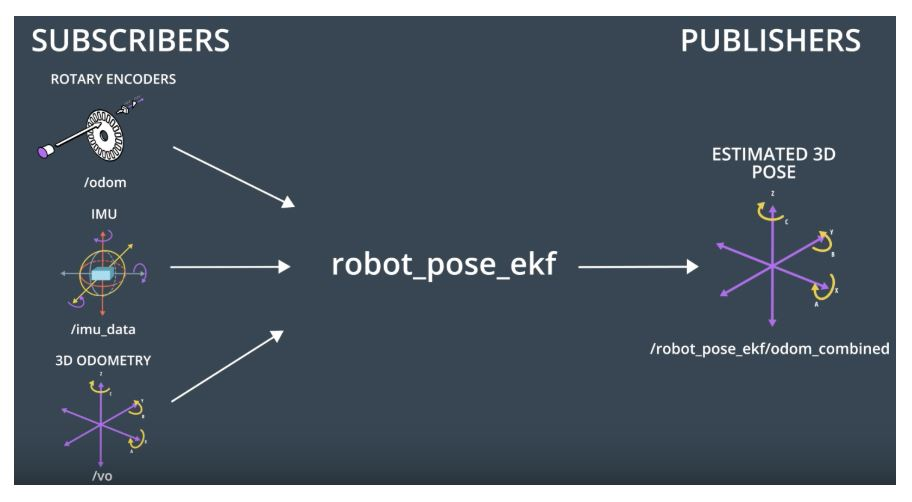
\includegraphics[width=.9\textwidth]{images/Alaa/rosPackage.JPG}%
     % you need to add the caption for the list of figures
    \caption[robot pose ekf packge]{The "robot\_pose\_ekf" package structure.}\label{fig: robot pose ekf packge}%
  \end{figure}
  
  
\subsubsection{Tuning Parameters}
\hspace{2cm} 
first, in order to match the package with our robot, we changed the covariance matrices of the sensors which represent the uncertainty of sensor's readings to some values that suit our sensor's readings.
\par 
\textbf{Hint}: we add such a big value (e.g. 9999) in the covariance matrix in the dimension that is ignored by the sensor. For example if wheel odometry is not giving a reading in Z direction then add to this cell a big number to be ignored.

\par
Second, we replace visual odometry by GPS sensor. A GPS sensor measures the robot 3d position, but not its orientation. The odometry message sent by the GPS sensor could look something like this:

 \begin{figure}[H]%
    \center%
    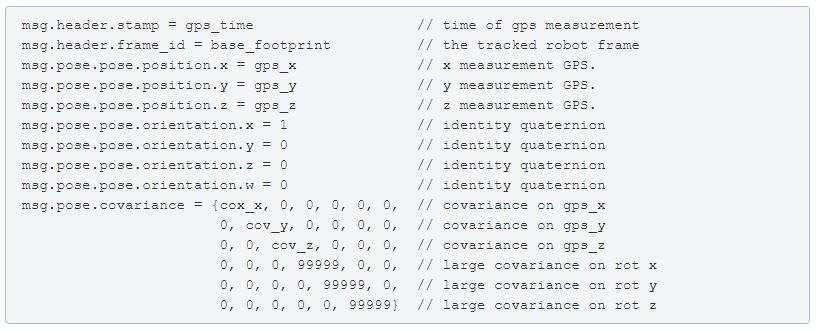
\includegraphics[width=1.0\textwidth]{images/Alaa/gps.JPG}%
     % you need to add the caption for the list of figures
    \caption[GPS message]{GPS message.}\cite{web037}\label{fig: GPS message}%
  \end{figure}


\section{Learning-based Follow Lane Controller} \label{learn}

\hspace{2cm} Convolutional Neural Networks, or CNNs, were designed to map image data to an output variable.
They have proven so effective that they are the go-to method for any type of prediction problem involving image data as an input.
as we depends mainly on the frames taken by the camera for the learning process,the CNN will be so effective.

Unlike neural networks, where the input is a vector, here the input is a multi-channeled image (3 channeled in this case).

But let us first understand what convolution mean:

We take the 5*5*3 filter and slide it over the complete image and along the way take the dot product between the filter and chunks of the input image shown in fig \ref{fig: Convolving an image with a filter}. \newline

\begin{figure}[H]%
 \center
	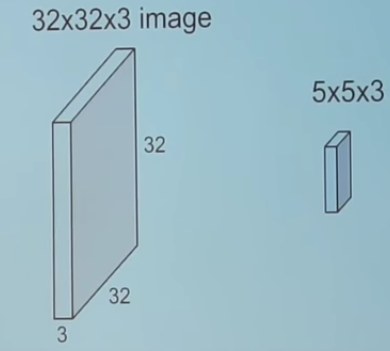
\includegraphics[width=.4\textwidth]{images/Learningprocess/Convolve.png}
    \caption[Convolving an image with a filter]{Convolving an image with a filter}\label{fig: Convolving an image with a filter}%
  \end{figure}
  
We take the 5*5*3 filter and slide it over the complete image and along the way take the dot product between the filter and chunks of the input image.
For every dot product taken, the result is a scalar.
Now, back to CNNs The convolution layer is the main building block of a convolutional neural network.

\begin{figure}[H]%
    \center
	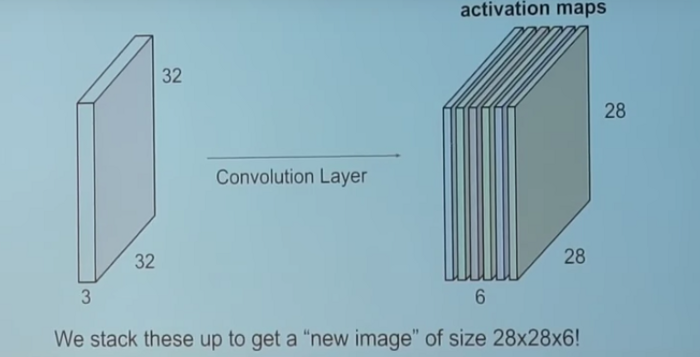
\includegraphics[width=.4\textwidth]{images/Learningprocess/layer.png}
    \caption[Convolution Layer]{Convolution Layer}\label{fig: Convolution Layer}%
\end{figure}
  
 Suppose we have a number of convolution layers in sequence.
 All these filters are initialized randomly and become our parameters which will be learned by the network subsequently.
 
 Take a look at \ref{fig: Filters in a trained network} the filters in the very first layer (these are our 5*5*3 filters). Through back propagation, they have tuned themselves to become blobs of coloured pieces and edges. As we go deeper to other convolution layers, the filters are doing dot products to the input of the previous convolution layers. So, they are taking the smaller coloured pieces or edges and making larger pieces out of them.
 
\ref{fig: Filters in a trained network}. 
\begin{figure}%
    \center
	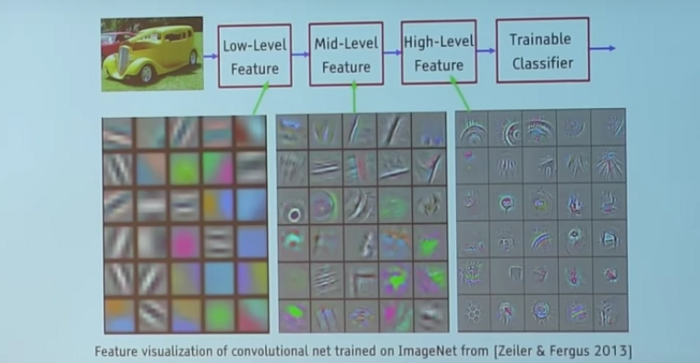
\includegraphics[width=1\textwidth]{images/Learningprocess/nn.png}
	
    \caption[Filters in a trained network]{Filters in a trained network}\label{fig: Filters in a trained network}%
\end{figure}
 
\subsection{Environment}
\subsubsection{World Setup}
\hspace{2cm}The environment composed of a map that satisfies different driving situations and multiple intersections to simulate a real road, the robot-to-map road ratio is the same as the a real car-to-real road ratio as shown in fig \ref{fig: World}. 


\begin{figure}%
\center
    \begin{minipage}[t]{0.3\linewidth}
	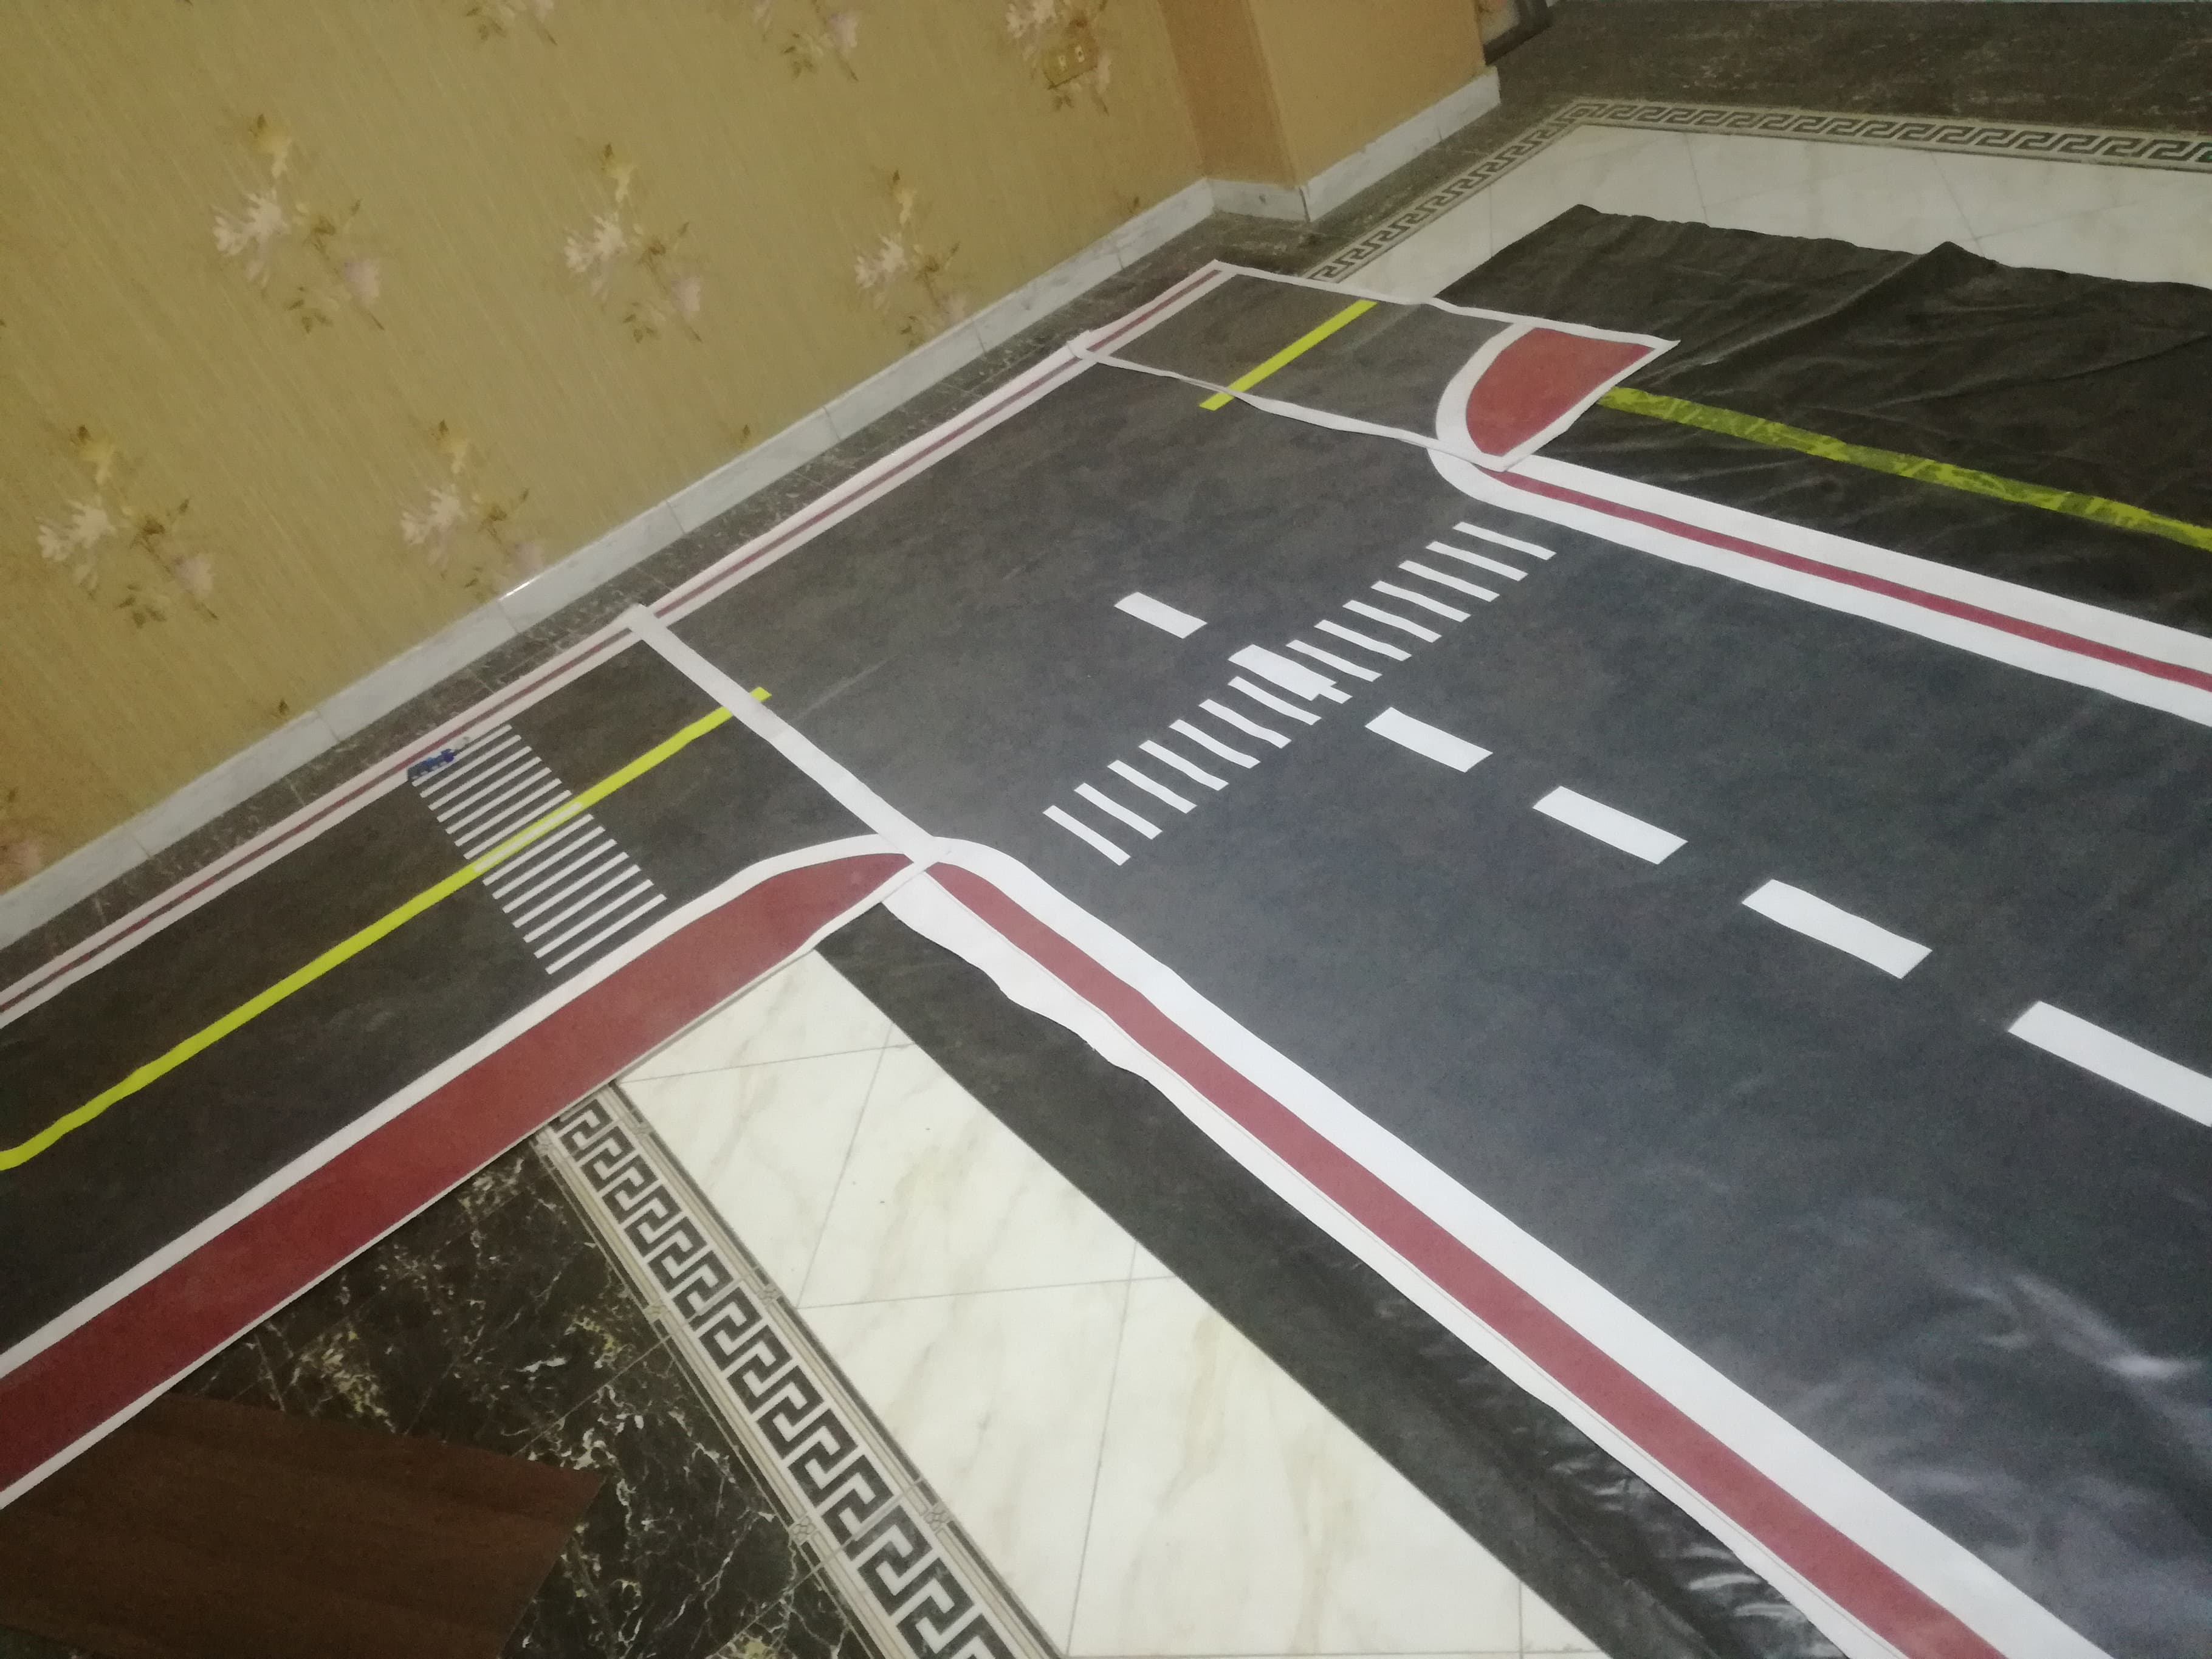
\includegraphics[width=\textwidth]{images/Learningprocess/world2.jpg}
     \end{minipage}
	\begin{minipage}[t]{0.3\linewidth}
	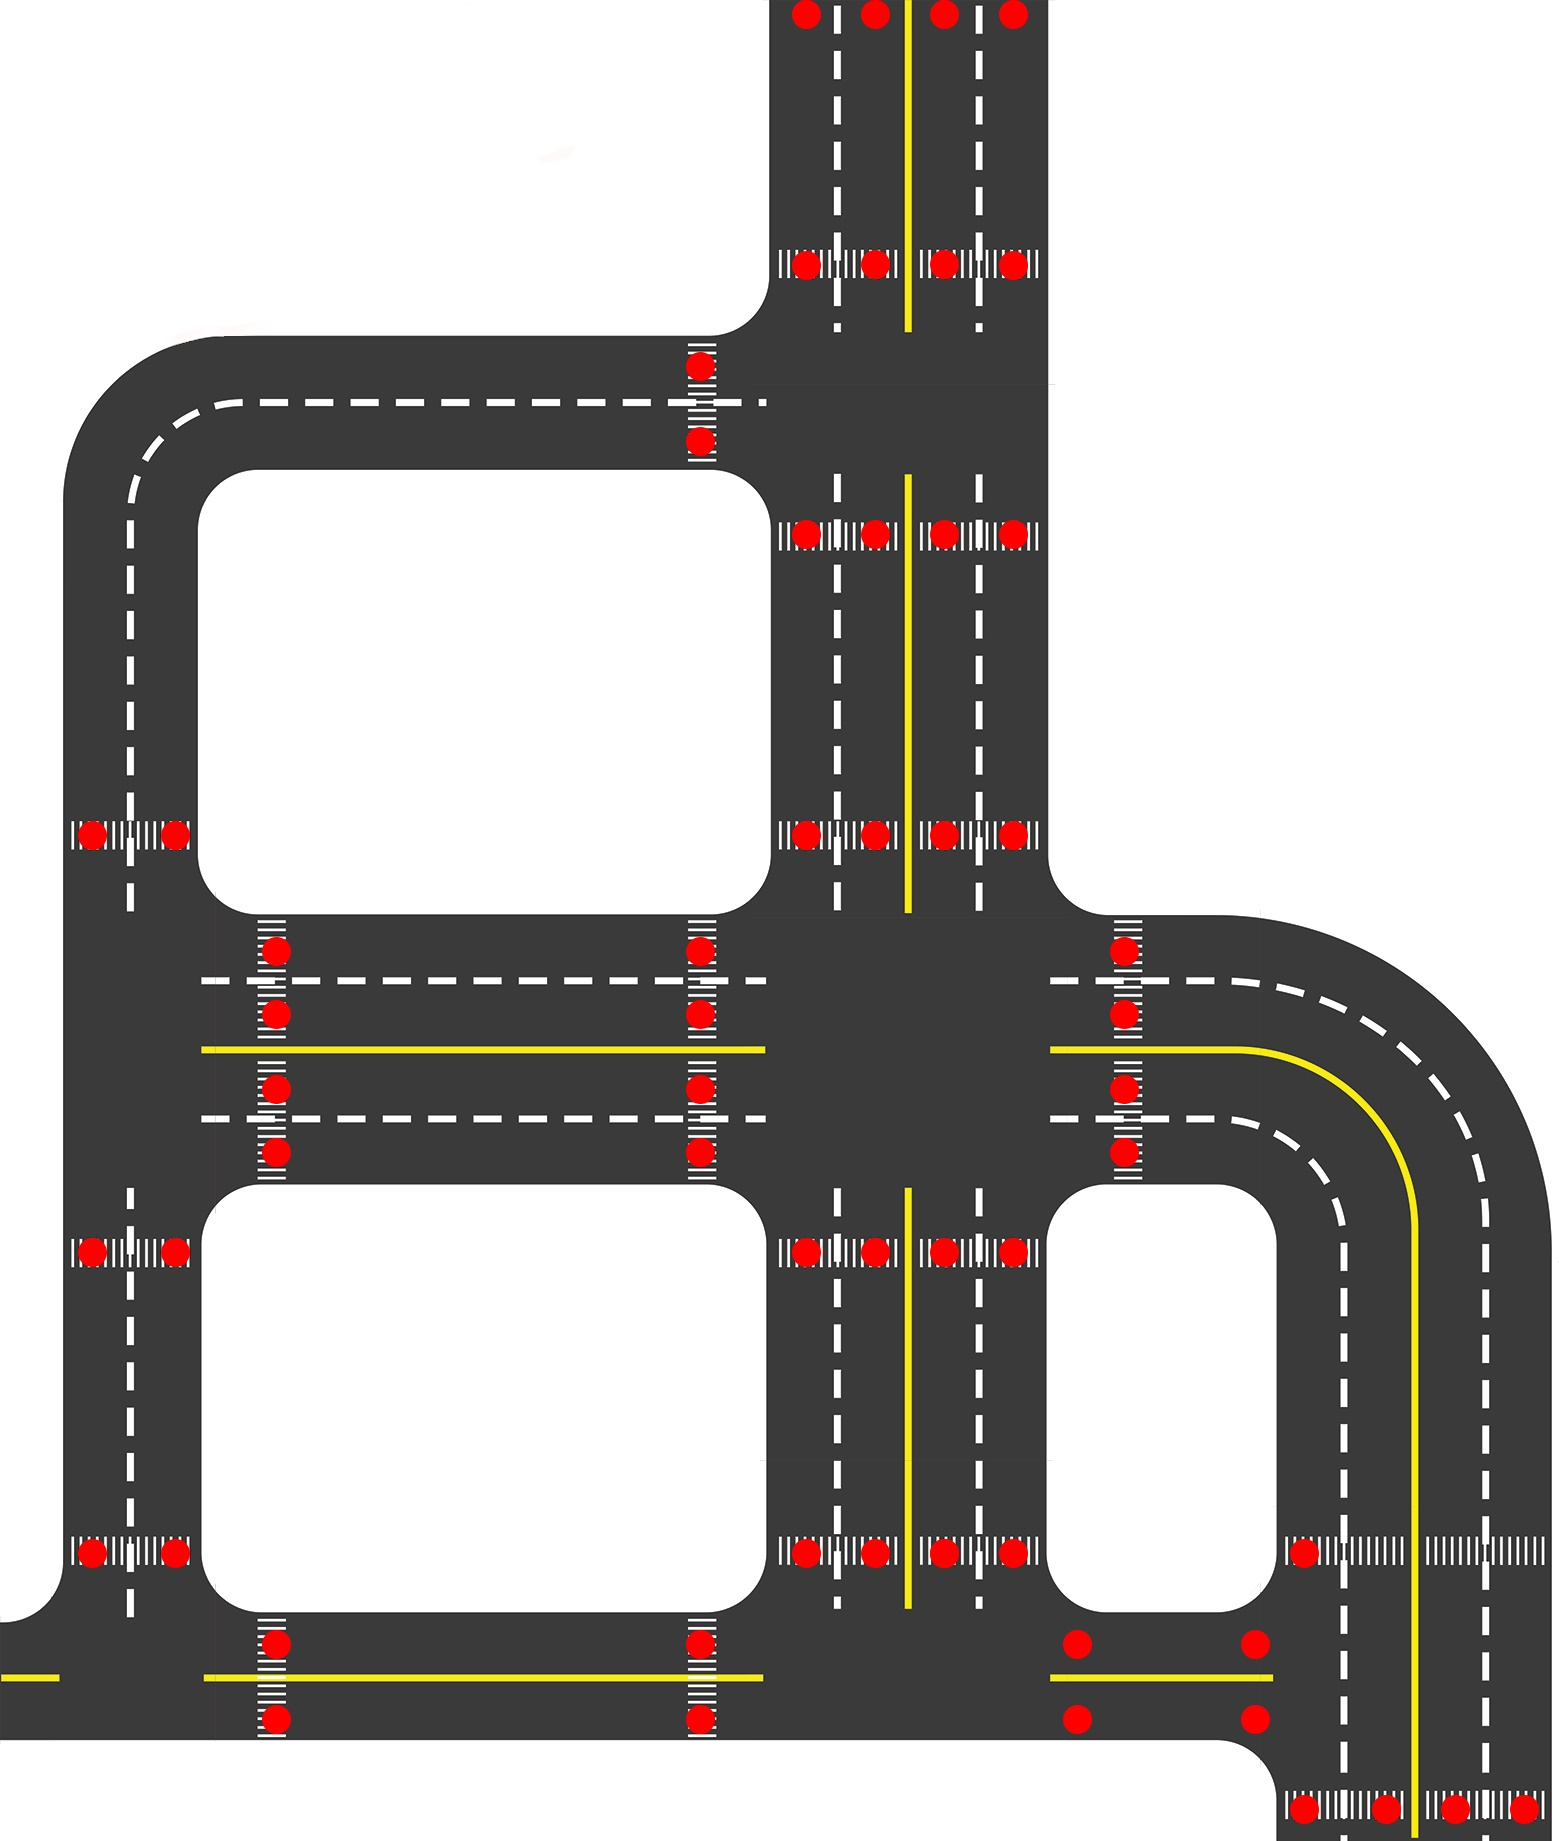
\includegraphics[width=\textwidth]{images/motion/map.jpg}
	\end{minipage}
    \caption[World]{World}\label{fig: World}%
  \end{figure}


\subsubsection{Car Sensors Setup}
\hspace{2cm} Our learning process depends mainly on a RGB Camera to deliver the scene information to The model.
the base of the camera is positioned 14cm in y-axis looking down with 10 degrees angle as shown in fig  \ref{fig: Camera}.

\begin{figure}%
    \center%
    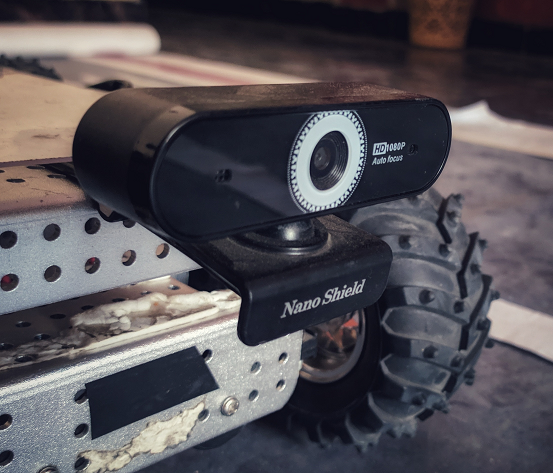
\includegraphics[width=.6\textwidth]{images/Learningprocess/small.png}%
     % you need to add the caption for the list of figures
    \caption[Camera]{Camera}\label{fig: Camera}%
 \end{figure}
 
\subsubsection{Software Environment Setup}
   \hspace{2cm} we use python3-OpenCV package used  for recording and manipulation of the images along side with h5py to save them with extension hdf5.
    we also used keras with back-end tensor-flow==10.13.1 for model construction, training and prediction.
    
\subsubsection{Data Generation}
 \hspace{2cm}During data collection the robot is driven by a human using keyboard and the camera is streaming images, control actions is then synchronized with camera images, then we saved it on the disk image with it's corresponding control actions.
 we started by collecting about 19k images for different scenes and actions in different lights.
 (fig \ref{fig: Data examples})
 
 \begin{figure}%
 \center
 \begin{minipage}[t]{0.3\linewidth}
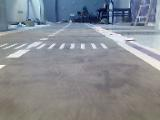
\includegraphics[width=\textwidth]{images/Learningprocess/1.jpg}
 \end{minipage}
\begin{minipage}[t]{0.3\linewidth}
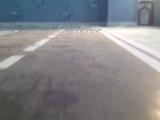
\includegraphics[width=\textwidth]{images/Learningprocess/2.jpg}
\end{minipage}
	\begin{minipage}[t]{0.3\linewidth}
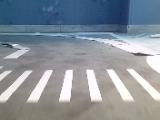
\includegraphics[width=\textwidth]{images/Learningprocess/3.jpg}
\end{minipage}
\begin{minipage}[t]{0.3\linewidth}
    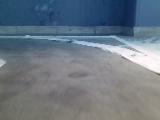
\includegraphics[width=\textwidth]{images/Learningprocess/4.jpg}
\end{minipage}
	\begin{minipage}[t]{0.3\linewidth}
\includegraphics[width=\textwidth]{images/Learningprocess/5.jpg}
\end{minipage}	\begin{minipage}[t]{0.3\linewidth}
\includegraphics[width=\textwidth]{images/Learningprocess/6.jpg}
\end{minipage}
  \caption[Data examples]{Data examples}\label{fig: Data examples}%
 \end{figure}
\subsubsection{Data Preprocessing}
\begin{enumerate}
    \item For making convergence faster while training the network. Data normalization is done by subtracting the mean from each pixel and then dividing the result by 255.
    \item for the variation and enhancement of the  learning process we start by shuffling all the data with their actions, Shuffling made sure that both train and validation set has data from all different driving conditions like daylight.
    \item for the validation and generalization of the  learning process after the  whole data was shuffled and then split into the train (80\%) and the validation set (20\%)
    \item we defines our ROI by cutting 20 pixels from the top.
    \item the last step was re sizing the images to 120*166.
    (fig \ref{fig: Data preprocessing})
    \begin{figure}%
    \begin{minipage}[t]{0.3\linewidth}
	\includegraphics[width=\textwidth]{images/Learningprocess/img3.png}
	\caption[camera photo]{ \left  \newline camera photo}
     \end{minipage}
	\begin{minipage}[t]{0.3\linewidth}
	\includegraphics[width=\textwidth]{images/Learningprocess/img4.png}
	\caption[ROI]{ \left \newline ROI}
	\end{minipage}
		\begin{minipage}[t]{0.3\linewidth}
	\includegraphics[width=\textwidth]{images/Learningprocess/img2.png}
	\caption[resized Image]{\left \newline \center re-sized Image}
	\end{minipage}
 	\caption[Data preprocessing]{ \center Data preprocessing} \label{fig: Data preprocessing}%
  \end{figure}
\end{enumerate}
\subsection{Data Analysis and Balancing}
\hspace{2cm}During data collection we make sure that data is balanced or not, thi  s could be done by calculating the number of images we took for every possible variation of the data, for example the number of curves, straight lines, cross sections and other possibilities.


\ref{fig: Camera}.
\begin{figure}%
    \center%
    \includegraphics[width=.2\textwidth]{images/Learningprocess/small.png}%
     % you need to add the caption for the list of figures
    \caption[Camera]{Camera}\label{fig: Camera}%
 \end{figure}
\subsection{Neural Network Model}

\subsubsection{Model Architecture}
\hspace{2cm}we picked up two different models for training
    \begin{enumerate}
        \item Donkey car linear model shown in fig \ref{fig: Donkey Car Model Architecture}.
         \item conditional imitation learning model
    \end{enumerate}

\begin{figure}%
    \center%

      \includegraphics[width=.3\textwidth]{images/Learningprocess/model.png}%
    \caption[Donkey Car Model Architecture]{Donkey Car Model Architecture}\label{fig: Donkey Car Model Architecture}%
 \end{figure}

 \begin{figure}%
  \includegraphics[width=1\textwidth]{images/Learningprocess/carla.png}%
     \caption[conditional imitation learning model]{ conditional imitation learning model}\label{fig:  conditional imitation learning model}%
  \end{figure}
each model have different learning process and architecture resulting in different accuracy, training time and losses.
\subsubsection{Model Training}
\hspace{2cm}when  we started the training process with early step option activated on the donkey car ,the model continued training until reaching 33 epochs of 100  the loss decreased  from loss .8 stepping down until reaching 0.015380 and stopped decreasing subsequently the training.
shown in (fig\ref{5.19}

for conditional imitation learning model training, the model continued training for 100 epochs reaching .001 loss and stopped decreasing.
 \begin{figure}%
 \begin{minipage}[t]{.3\linewidth}
    \center
    \includegraphics[width=1\textwidth]{images/Learningprocess/lossGraph.png}%

     % you need to add the caption for the list of figures
    \end{minipage}
    \begin{minipage}[t]{.5\linewidth}
    \includegraphics[width=1\textwidth]{images/Learningprocess/carla-valid.png}%
\caption[model losses]{ model losses}\label{fig:  model losses}%
     % you need to add the caption for the list of figures
    \end{minipage}
    
      \end{figure}
\subsubsection{Model Prediction and Output Mapping}

\hspace {2cm}both imitation model and donkey model has achieved good accuracy and low loss after training, the biggest challenge in the process is to run the model on a device that has a good enough requirement that satisfies the running requirements.
for donkey car model prediction we used the raspberry pi 3 b+ for running which achieved reasonable performance with average of 15 frame predicted in second

for imitation learning we used a pc setup with a connected socket with the raspberry bi achieving average of 15 frame predicted in second.
both models has achieved a very good accuracy and low loss.
(fig \ref{fig:  model losses})
%%%%%%%%%%%%%%%%%%%%%%%%%%%%%%%%%%%%%%%%%%%%%%%%%%%%%%%%%%%%%%%%%%%%%%%%%%%%%%%%%%%%%%%%%%%%%%%%%%%%%%%%%%%%%%%%%%

     \cleardoublepage%
     
     %%%%%%%%%%%%%%%%%%%%%%%%%%%%
% CHAPTER                  %
%%%%%%%%%%%%%%%%%%%%%%%%%%%%
\chapter{Web and Mobile Application}%
\label{chap:chap6}



%%%%%%%%%%%%%%%%%%%%%%%%%%%%
% SECTION                  %
%%%%%%%%%%%%%%%%%%%%%%%%%%%%
\newline
\newline
\vspace{3mm}
\hfill

\section{Introduction}

\hspace{2cm}In this chapter we discuss software architecture in the project, services, back-end and front-end architecture.
Web services are used in communication between users (customers and vendors) of the website and mobile application and the robot.
By sending a request to the server containing specific data then waiting for the appropriate response to send it to the robot server to perform the wanted action which will be a position the robot will go to.
We will describe the functionality of each part of the software system, including database to store the users, order, vendor’s products and robot location.


\section{Software Architecture}
\hspace{2cm}This Diagram Describe Software Architecture of our web site \ref{fig: LMD}
\begin{figure}%
    \center%
    \includegraphics[width=1\textwidth]{images/Software/frontend.png}%
     % you need to add the caption for the list of figures
    \caption[LMD Software Architecture]{LMD Software Architecture}\label{fig: LMD}%
  \end{figure}

 
\begin{figure}[htp]%
    \center%
    \includegraphics[width=1\textwidth]{images/Software/backend1.png}%
     % you need to add the caption for the list of figures
    \caption[Back End]{Back End}\label{fig: Back End}%
  \end{figure}




\section{Back-end Architecture}
\hspace{2cm}Back-end is all of the technology required to process the incoming request and generate and send the response to the client. This typically includes three major parts:
    \begin{enumerate}
    \setcounter{enumi}{0}
    \item Server that receives the request.
    \item Application. This is the application running on the server that listens for the requests, retrieve the data from the database and send the response to the user.
    \item Database that is used to store and organize the data
    \end{enumerate}
    
We use NodeJs write the server side application which is an open-source, cross-platform JavaScript run-time environment that executes JavaScript code outside of a browser to produce dynamic web page content before the page is sent to the user's web browser.
Express package is a minimal and flexible Node.js web application framework that provides a robust set of features for web and mobile applications. We use it  to  set up middlewares, to respond to HTTP Requests to Define a routing table which is used to perform different actions based on HTTP Method and URL 
and to dynamically render HTML Pages based on passing arguments to templates.

\subsection{Server}
\hspace{2cm}Is a computer designed to process requests and deliver data to another computer, called “Clients ” over the internet or a local network, This architecture called client-server model. In this model server serve the data from client.

The nature of communication between server and client  in “request-and-response”.
\begin{figure}%
    \center%
    \includegraphics[width=1\textwidth]{images/Software/clientserver.png}%
     % you need to add the caption for the list of figures
    \caption[Client and Server Communication]{Client and Server Communication}\label{fig: login}%
  \end{figure}
  
 Server runs an app that contains logic about how to respond to various requests based on the HTTP verb and the Uniform Resource Identifier (URI). The pair of an HTTP verb and a URI is called a route and matching them based on a request is called routing.
The data that the server sends back can come in different forms. For example, a server might serve up an HTML file, send data as JSON, or it might send back only an HTTP status code. You’ve probably seen the status code “404 - Not Found” whenever you’ve tried navigating to a URI that doesn’t exist.

\subsection{Application Architecture}
\hspace{2cm}Web application development uses a 3-tiers MVC (model-view-controller) design pattern.it provide three main layers; model, view , controller. MVC pattern separates the characteristic of the application which makes it easy for us to test our application as relation among different components of the application. These tiers describe as shown in figure
\begin{figure}%
    \center%
    \includegraphics[width=1\textwidth]{images/Software/MVC2.png}%
     % you need to add the caption for the list of figures
    \caption[Web based application]{Web based application}\label{fig: login}%
  \end{figure}
\begin{enumerate}
    \setcounter{enumi}{0}
    \item Model :- Model component corresponds to all the data-related logic that the user works with. This can represent either the data that is being transferred between the View and Controller components or any other business logic-related data. It is used to retrieve, insert or update the data into the database associated with our application. An example of the code to connect to the database is given below :
\begin{figure}%
    \center%
    \includegraphics[width=1\textwidth]{images/Software/Capture.PNG}%
     % you need to add the caption for the list of figures
    \caption[Database Communication]{Database Communication}\label{fig: login}%
  \end{figure}
  
    \item View:- in a web-based application is representation of the user-interface (UI). Buttons, forms and other information visible to the user on the web are all part of View.  By using that interface users interact with our application. These Views are generally bind from the model data and have extensions such as html, aspx, cshtml,
    vbhtml, etc.
    
    \item Controllers:- act as an interface between Model and View components to process all the business logic and incoming requests, manipulate data using the Model component and interact with the Views to render the final output. So when the user clicks on the hyperlinks in the web page , the controlled receive the request and determine which model to call, and it confirms to use which view to display the returning data of the model processing.
    \end{enumerate}  

 
 Our website has many controllers:
  \begin{enumerate}
    \setcounter{enumi}{0}
    \item Customers Controller: uses many apis to get and update and delete and create new customer in our system. Apis are:
    \begin{itemize}
    \item GET /api/customers: To get all customer 

    \item POST /api/customers: To create new Customers

     \item DELETE /api/customers/:id: To delete Customers \newline
    \end{itemize} 

    \item Vendors Controller: uses many apis to get and update and delete and create new Vendor in our system. Apis are :
    \begin{itemize}
    \item GET /api/vendors: To get all Vendors 

    \item POST /api/vendors: To create new Vendors

     \item DELETE /api/vendors/:id: To delete Vendors
     
     \item PUT /api/vendors/:id: To update specific vendor \newline

    \end{itemize}
    
    \item Products Controller: uses many apis to get all products and update the data of a product of specific vendor,delete a product of specific vendor and create new products to the chosen vendor. 
	Apis are :
	\begin{itemize}
    \item GET /api/products: To get all products
    \item POST /api/products: To Create new product
     \item DELETE /api/products/:id: To delete product of specific vendor
     \item PUT /api/products/:id: To update product of specific vendor \newline
    \end{itemize} 

    \item Orders Controller: uses many apis to get all orders made by the users, update and delete the data of orders before it being shipped to customer, and create new orders that included many products of the vendors in our system.
    \begin{itemize}
    \item GET /api/orders: To get all Orders
    \item POST /api/orders: To Create new Orders
     \item DELETE /api/orders/:id: To delete specific Order
     \item PUT /api/orders/:id: To update specific Orders
     \newline
    \end{itemize} 
    
    \item Robot Controller: will be used in the future when we have more than one Robot. Each robot will have unique ID. So when we make an order, routing algorithm can be used to choose the free and the nearest robot to deliver the order.\newline
    
    \item Cart Controller: is used to get all items Which has been selected for purchase by specific user. it is used also to add new items or delete items from the cart of the authenticated user. \newline

    \item Payment Controller: will allow individuals and businesses to make and receive payments over the Internet. It will provide the technical, fraud prevention, and banking infrastructure required to operate online payment systems.\newline

    \item Users Controller: gets all users in our system included vendors and customers.\newline
    
    \item Authentication Controller: allows users to log in to the system. So when user enters the E-mail and the password, post request is used to check the Data in the body of the request to verify the user.
Once user is logged in, each request will include token, allowing the user to access routes, services, and resources that are permitted with that token. 
Authentication can be made by many methods, in our system authentication is made using JSON Web Token (JWT).\newline \hfill \break
\textbf{JSON Web Token} (\textbf{JWT}) \cite{JWT}:
is an open standard (RFC 7519) that defines a compact and self-contained way for securely transmitting information between parties as a JSON object. This information can be verified and trusted because it is digitally signed. JWTs can be signed using a secret (with the \textbf{HMAC} algorithm) or a public/private key pair using \textbf{RSA} or \textbf{ECDSA}.\newline
JSON Web Tokens looks like the following: xxxxx.yyyyy.zzzzz and consists of three parts separated by dots (.) which are:
\begin{enumerate}
    \setcounter{enumi}{0}
    \item Header: typically consists of two parts: the type of the token, which is JWT, and the signing algorithm being used, such as HMAC SHA256 or RSA
    \item Payload: contains the claims. Claims are statements about an entity (typically, the user) and additional data. There are three types of claims: registered, public, and private claims.
    \item Signature: To create the signature part you have to take the encoded header, the encoded payload, a secret, the algorithm specified in the header, and sign that. The signature is used to verify the message wasn't changed along the way, and, in the case of tokens signed with a private key, it can also verify that the sender of the JWT is who it says it is.
    The figure \ref{fig: jwt} shows a JWT that has the header and payload encoded, and it is signed with a secret.
    \begin{figure}[htp]%
    \center%
    \includegraphics[width=1\textwidth]{images/Software/encoded-jwt3.png}%
     % you need to add the caption for the list of figures
    \caption[Encoded JWT]{Encoded JWT}\label{fig: jwt}%
  \end{figure}
    \end{enumerate}
    In figure \ref{fig: djwt} you can use decode JWT to  know the additional data about the user, and to define the type of the token.
 \begin{figure}[htp]%
    \center%
    \includegraphics[width=1\textwidth]{images/Software/legacy-app-auth-5.png}%
     % you need to add the caption for the list of figures
    \caption[Encoded and Decoded JWT]{Encoded and Decoded JWT}\label{fig: djwt}%
  \end{figure}
    \end{enumerate} \newpage
    
\subsection{Database Architecture}
\hspace{2cm}This section illustrates the architecture of the database using NoSQL database. The figure \ref{fig: db schema} describes the tables created in the database. Each table has a primary key and a foreign key to connect to another table.
We used MongoDB is a cross-platform document-oriented database program. Classified as a NoSQL database program, MongoDB uses JSON-like documents with schema. Also Fields in a MongoDB document can be indexed with primary and secondary indices.
To validate the entered data we used Joi. Joi allows you to create blueprints or schemas for JavaScript objects (an object that stores information) to ensure validation of key information.
We define the input must be a string, number.. etc, if the input is required or not, if there is a specified regular expression such as emails and passwords.
\begin{figure}[htp]%
    \center%
    \includegraphics[width=1\textwidth]{images/Software/dbSchema.jpeg}%
     % you need to add the caption for the list of figures
    \caption[DataBase Shcema]{DataBase Shcema}\label{fig: db schema}%
  \end{figure} \newpage
  

\section{Web Application Front-end}
\hspace{2cm}Front-end web development, also known as client-side development is the practice of producing HTML, CSS and JavaScript for Web Application so that a user can see and interact with them directly. 

We use React.Js which is a JavaScript library for building user interfaces as the basic architecture of React applies beyond rendering HTML element in the browser.
React applications usually require the use of additional libraries for state management, routing, and interaction with an API such as: semantic-ui which is framework designed for theming and axios HTTP requests from both browser and server. Axios is an npm library (originally short for Node Package Manager) is a package manager for the JavaScript programming language.

One of the advantages to use React is the use of a "virtual Document Object Model", or "virtual DOM". React creates an in-memory data-structure cache, computes the resulting differences, and then updates the browser's displayed DOM efficiently. This allows the programmer to write code as if the entire page is rendered on each change, while the React libraries only render subcomponents that actually change.

Now, we will add routes to the app. This time the Router will be rendered. We will also set components for each route.

As shown in figure \ref{fig: routes} we have these routes in the website.
\begin{figure}[htp]%
    \center%
    \includegraphics[width=1\textwidth]{images/Software/routes.PNG}%
     % you need to add the caption for the list of figures
    \caption[Website Routes]{Website Routes}\label{fig: routes}%
  \end{figure}

\textbf{Website Pages} 
In Figure \ref{fig: login} a login page to enter the email and password also checks that the user must be authorized.
\begin{figure}[htp]%
    \center%
    \includegraphics[width=1\textwidth]{images/Software/login.PNG}%
     % you need to add the caption for the list of figures
    \caption[Website: Login page]{Website: Login page}\label{fig: login}%
  \end{figure}

In Figure \ref{fig: main Page} main page contains our logo and top categories such as (Food, Health and Clothes), the user can access the shop, his cart or choose his favourite category.\newline \newline
\begin{figure}[htp]%
    \center%
    \includegraphics[width=1\textwidth]{images/Software/MainPage.PNG}%
     % you need to add the caption for the list of figures
    \caption[Website: Main Page]{Website: Main Page}\label{fig: main Page}%
  \end{figure}\newline \newline
 
In Figure \ref{fig: profile} profile page for the customer to be able to track his orders and recent activities. Also if the user is a vendor, "Add Product" button will be shown to enable him to add his products to be shown in the shop.
\begin{figure}[htp]%
    \center%
    \includegraphics[width=1\textwidth]{images/Software/profile.jpeg}%
     % you need to add the caption for the list of figures
    \caption[Website: Profile Page]{Website: Profile Page}\label{fig: profile}%
  \end{figure}\newpage
  
In Figure \ref{fig: vendors}, \ref{fig: products} and \ref{fig: product Page} shop page has our vendors each contains their products with description provided it product page, search and filter by category are available while browsing and from product page the user can add this product to his cart.

  \begin{figure}[htp]%
    \center%
    \includegraphics[width=1\textwidth]{images/Software/vendors.PNG}%
     % you need to add the caption for the list of figures
    \caption[Website: Vendors Page]{Website: Vendors Page}\label{fig: vendors}%
  \end{figure}
  
  \begin{figure}[htp]%
    \center%
    \includegraphics[width=1\textwidth]{images/Software/products.PNG}%
     % you need to add the caption for the list of figures
    \caption[Website: Products Page]{Website: Products Page}\label{fig: products}%
  \end{figure}\newline
  
    \begin{figure}[htp]%
    \center%
    \includegraphics[width=1\textwidth]{images/Software/productPage.PNG}%
     % you need to add the caption for the list of figures
    \caption[Website: product Page]{Product Page}\label{fig: product Page}%
  \end{figure}\newpage
  

In Figure \ref{fig: cart} each user has its own cart with different elements to buy the “proceed to check out” button redirects the user to Stripe component as shown in figure  \ref{fig: payment} that access his location and visa card to continue to checkout.
Stripe is an American technology company its software allows individuals and businesses to make and receive payments over the Internet. Stripe provides the technical, fraud prevention, and banking infrastructure required to operate online payment systems \cite{Stripe}.

\begin{figure}[htp]%
    \center%
    \includegraphics[width=1\textwidth]{images/Software/cart.PNG}%
     % you need to add the caption for the list of figures
    \caption[Website: Cart Page]{Website: Cart Page}\label{fig: cart}%
  \end{figure}
  
   \begin{figure}[htp]%
    \center%
    \includegraphics[width=1\textwidth]{images/Software/payment.PNG}%
     % you need to add the caption for the list of figures
    \caption[Website: Payment Page]{Website: Payment Page}\label{fig: payment}%
  \end{figure}\newpage

In figure \ref{fig: tracking} Tracking page is used to track the robot carrying the order with tracking password as shown in figure\ref{fig:trackPas}.
  \begin{figure}[htp]%
    \center%
    \includegraphics[width=1\textwidth]{images/Software/tracking.PNG}%
     % you need to add the caption for the list of figures
    \caption[Website: Tracking Page]{Tracking Page}\label{fig: tracking}%
  \end{figure}
  
    \begin{figure}[htp]%
    \center%
    \includegraphics[width=1\textwidth]{images/Software/trackingPassword.PNG}%
     % you need to add the caption for the list of figures
    \caption[Website: Tracking Password Page]{ Tracking Password Page}\label{fig:trackPas}%
  \end{figure}
  
Also the vendor has its own page to add his products as shown in figure \ref{fig: add Product}.
  \begin{figure}[htp]%
    \center%
    \includegraphics[width=1\textwidth]{images/Software/addProduct.PNG}%
     % you need to add the caption for the list of figures
    \caption[Website: Add Product Page]{Website: Add Product Page}\label{fig: add Product}%
  \end{figure} \newpage
  
At last, we have our page that defines the scope of the project and the team members as shown in figure \ref{fig: about1}
  \begin{figure}[htp]%
    \center%
    \includegraphics[width=1\textwidth]{images/Software/about1.PNG}%
     % you need to add the caption for the list of figures
    \caption[Website: About Page (i)]{Website:  About Page (i)}\label{fig: about1}%
  \end{figure}
   \begin{figure}[htp]%
    \center%
    \includegraphics[width=1\textwidth]{images/Software/about2.PNG}%
     % you need to add the caption for the list of figures
    \caption[Website: About Page (ii)]{Website:  About Page (ii)}\label{fig: about2}%
  \end{figure}
\section{Mobile Front-End}
\hspace{2cm}We use React  which is a JavaScript framework for writing real, natively rendering mobile applications for iOS and Android. It’s based on React, Facebook’s JavaScript library for building user interfaces,but instead of targeting the browser, it targets mobile platforms.

Similar to React for the Web, React Native applications are written using a mixture of JavaScript and XML-esque markup, known as JSX. Then, under the hood, the React Native “bridge” invokes the native rendering APIs in Objective-C (for iOS) or Java (for Android). Thus, your application will render using real mobile UI components, not webviews, and will look and feel like any other mobile application. React Native also exposes JavaScript interfaces for platform APIs, so your React Native apps can access platform features like the phone camera, or the user’s location \cite{React-native}.\newpage

\textbf{Mobile Screens}:
\newline
 In figure \ref{fig: homescreen} main page contains our logo and top categories such as (Food, Health and Clothes), the user can access the shop or choose his favourite category.

\begin{figure}[htp]%
    \center%
    \includegraphics[width=0.52\textwidth]{images/Software/Mainscreen.jpg}%
     % you need to add the caption for the list of figures
    \caption[Mobile Application: Home Screen]{Mobile Application: Home Screen}\label{fig: homescreen}%
  \end{figure}
  
  
In Figure \ref{fig: singin} a login Screen to enter the email and password also checks that the user must be authorized.it also contain sing up page if the user doesn't have account on our system.

\begin{figure}[htp]%
    \center%
    \includegraphics[width=0.52\textwidth]{images/Software/signin.jpg}%
     % you need to add the caption for the list of figures
    \caption[Mobile Application: Login Screen]{Mobile Application: Login Screen}\label{fig: singin}%
  \end{figure}
\newpage  


In Figure \ref{fig: singup} a Sing Up to register new user in our system.
\begin{figure}[htp]%
    \center%
    \includegraphics[width=0.5\textwidth]{images/Software/signup.jpg}%
     % you need to add the caption for the list of figures
    \caption[Mobile Application: Sing up Screen]{Mobile Application: Sing up Screen}\label{fig: singup}%
  \end{figure}
\newpage


In Figure \ref{fig: shop} shop Screen has our vendors in the system.
  \begin{figure}[htp]%
    \center%
    \includegraphics[width=0.5\textwidth]{images/Software/Shop.jpg}%
     % you need to add the caption for the list of figures
    \caption[Mobile Application: Shop Screen]{Shop Screen}\label{fig: shop}%
  \end{figure} \newpage
  
 In figure \ref{fig: productsscreen} Each Vendors have their products with description provided it product page in figure \ref{fig: productPageScreen} , search and filter by category are available while browsing and from product page the user can add this product to his cart.
  
  \begin{figure}[htp]%
    \center%
    \includegraphics[width=0.5\textwidth]{images/Software/productsscreen.jpg}%
     % you need to add the caption for the list of figures
    \caption[Mobile Application:Products Screen]{Products Screen}\label{fig: productsscreen}%
  \end{figure}
  
    \begin{figure}[htp]%
    \center%
    \includegraphics[width=0.5\textwidth]{images/Software/product.jpg}%
     % you need to add the caption for the list of figures
    \caption[Mobile Application: product Screen]{product Screen}\label{fig: productPageScreen}%
  \end{figure}\newpage
  
In Figure \ref{fig: Mobile Application:Cart Screen} each user has its own cart with different elements to buy the “proceed to check out” button redirects the user to Stripe component.  
\newline
\begin{figure}[htp]%
    \center%
    \includegraphics[width=0.44\textwidth]{images/Software/cartmobile.png}%
     % you need to add the caption for the list of figures
    \caption[Mobile Application:Cart Screen]{Mobile Application:Cart Screen}\label{fig: Mobile Application:Cart Screen}%
  \end{figure}
  
  
  


%%%%%%%%%%%%%%%%%%%%%%%%%%%%%%%%%%%%%%%%%%%%%%%%%%%%%%%%%%%%%%%%%%%%%%%%%%%%%%%%%%%%%%%%%%%%%%%%%%%%%%%%%%%%%%%%%%


     \cleardoublepage%
     
     %%%%%%%%%%%%%%%%%%%%%%%%%%%%
% CHAPTER                  %
%%%%%%%%%%%%%%%%%%%%%%%%%%%%
\chapter{Conclusions and Future Work}%
\label{chap:chap7}

%%%%%%%%%%%%%%%%%%%%%%%%%%%%
% SECTION                  %
%%%%%%%%%%%%%%%%%%%%%%%%%%%%
\newline
\newline
\vspace{3mm}
\hfill

\section{Conclusions}
\hspace{2cm}Automating the delivery process has been regarded as a significant topic in research due to its importance in real world applications. This project was our chance to leave a footprint in this topic and we concluded the following: The importance and the huge effect that ROS (Robot Operating System) has, Allowing us to remove and attach as many components to the system as we need, Making the system flexible and easily scalable, also facilitating module-to-module communication lifting up the overhead of implementing reliable communication modules, Leaving up to focus on our main work. The possibility of implementing a controller that is a mixture of both: Classical and Neural Network modules without the need of implementing a full end-to-end controller at the moment, as the implementation of end-to-end controller would require more time and huge amount of data to be collected.
\section{Future Work}
\hspace{2cm}For the future we have in mind multiple ideas, that could be put in motion to improve our current system's service, In this section we introduce some of these ideas from both: technical and business point of views.\\
\textbf{Technical-wise}\\
From technical point of view we can improve our system by achieving the following:
\begin{enumerate}
    \item Implementation of a subtle vehicle-to vehicle communication to propagate information faster through the system.
    \item Improving the current database to handle vast number of mobile robots operating at the same time.
    \item Modifying the robot to work in more chaotic environment by implementing full end-to-end robot 
    controllers. 
    \item Reducing the time of delivery by increasing the accuracy of both the path planning and the neural network modules.
    \item Enhancing the quality of our customers' service by adding more features to the currently used E-commerce system (Website and Mobile Application).
\end{enumerate}
\newpage
\textbf{Business-wise}\\
From business point of view we can improve our business by achieving the following:
\begin{enumerate}
    \item Building a fleet of self-driving robots, Covering a wider delivery zone subsequently increasing our service availability.
    \item Deploying our system to a production suitable components instead of the currently used high-cost development components. 
    \item Attracting more vendors to contract with us to use or service in selling and delivering their products. 
    \item Building a concrete long-term marketing strategy to spread the acceptance of self-driving robots and increase our customers base.
\end{enumerate}
%%%%%%%%%%%%%%%%%%%%%%%%%%%%%%%%%%%%%%%%%%%%%%%%%%%%%%%%%%%%%%%%%%%%%%%%%%%%%%%%%%%%%%%%%%%%%%%%%%%%%%%%%%%%%%%%%%
     \cleardoublepage%

     \appendix
    \chapter{Appendix: Project Code}
    \textbf{All project work is found in the following gitHub link:}

\url{https://github.com/lastmiledeliverysystem}

    
     %%%%%%%%%%%%%%%%%%%%%%%%%%%%%%%%%%%%%%%%%%%%%%%%%%%%
% Don't touch this, it is auto generated
%%%%%%%%%%%%%%%%%%%%%%%%%%%%%%%%%%%%%%%%%%%%%%%%%%%%
\nocite{*}

\phantomsection{}
\addcontentsline{toc}{chapter}{References}
\printbibliography[title={References},type=online]   %%chapter name

%\phantomsection{}
%\addcontentsline{toc}{chapter}{References}
%\printbibliography[title={References},nottype=online]
     \cleardoublepage%
     
   


    \addtocontents{toc}{\protect\setcounter{tocdepth}{3}}
    
   
  \end{mrs-doc-tanta}
\end{document}